% From https://github.com/UWIT-IAM/UWThesis

\documentclass [11pt, proquest] {uwthesis}[2015/03/03]

% Syntax highlighting #22
  \usepackage{color}
  \usepackage{fancyvrb}
  \newcommand{\VerbBar}{|}
  \newcommand{\VERB}{\Verb[commandchars=\\\{\}]}
  \DefineVerbatimEnvironment{Highlighting}{Verbatim}{commandchars=\\\{\}}
  % Add ',fontsize=\small' for more characters per line
  \usepackage{framed}
  \definecolor{shadecolor}{RGB}{248,248,248}
  \newenvironment{Shaded}{\begin{snugshade}}{\end{snugshade}}
  \newcommand{\KeywordTok}[1]{\textcolor[rgb]{0.13,0.29,0.53}{\textbf{#1}}}
  \newcommand{\DataTypeTok}[1]{\textcolor[rgb]{0.13,0.29,0.53}{#1}}
  \newcommand{\DecValTok}[1]{\textcolor[rgb]{0.00,0.00,0.81}{#1}}
  \newcommand{\BaseNTok}[1]{\textcolor[rgb]{0.00,0.00,0.81}{#1}}
  \newcommand{\FloatTok}[1]{\textcolor[rgb]{0.00,0.00,0.81}{#1}}
  \newcommand{\ConstantTok}[1]{\textcolor[rgb]{0.00,0.00,0.00}{#1}}
  \newcommand{\CharTok}[1]{\textcolor[rgb]{0.31,0.60,0.02}{#1}}
  \newcommand{\SpecialCharTok}[1]{\textcolor[rgb]{0.00,0.00,0.00}{#1}}
  \newcommand{\StringTok}[1]{\textcolor[rgb]{0.31,0.60,0.02}{#1}}
  \newcommand{\VerbatimStringTok}[1]{\textcolor[rgb]{0.31,0.60,0.02}{#1}}
  \newcommand{\SpecialStringTok}[1]{\textcolor[rgb]{0.31,0.60,0.02}{#1}}
  \newcommand{\ImportTok}[1]{#1}
  \newcommand{\CommentTok}[1]{\textcolor[rgb]{0.56,0.35,0.01}{\textit{#1}}}
  \newcommand{\DocumentationTok}[1]{\textcolor[rgb]{0.56,0.35,0.01}{\textbf{\textit{#1}}}}
  \newcommand{\AnnotationTok}[1]{\textcolor[rgb]{0.56,0.35,0.01}{\textbf{\textit{#1}}}}
  \newcommand{\CommentVarTok}[1]{\textcolor[rgb]{0.56,0.35,0.01}{\textbf{\textit{#1}}}}
  \newcommand{\OtherTok}[1]{\textcolor[rgb]{0.56,0.35,0.01}{#1}}
  \newcommand{\FunctionTok}[1]{\textcolor[rgb]{0.00,0.00,0.00}{#1}}
  \newcommand{\VariableTok}[1]{\textcolor[rgb]{0.00,0.00,0.00}{#1}}
  \newcommand{\ControlFlowTok}[1]{\textcolor[rgb]{0.13,0.29,0.53}{\textbf{#1}}}
  \newcommand{\OperatorTok}[1]{\textcolor[rgb]{0.81,0.36,0.00}{\textbf{#1}}}
  \newcommand{\BuiltInTok}[1]{#1}
  \newcommand{\ExtensionTok}[1]{#1}
  \newcommand{\PreprocessorTok}[1]{\textcolor[rgb]{0.56,0.35,0.01}{\textit{#1}}}
  \newcommand{\AttributeTok}[1]{\textcolor[rgb]{0.77,0.63,0.00}{#1}}
  \newcommand{\RegionMarkerTok}[1]{#1}
  \newcommand{\InformationTok}[1]{\textcolor[rgb]{0.56,0.35,0.01}{\textbf{\textit{#1}}}}
  \newcommand{\WarningTok}[1]{\textcolor[rgb]{0.56,0.35,0.01}{\textbf{\textit{#1}}}}
  \newcommand{\AlertTok}[1]{\textcolor[rgb]{0.94,0.16,0.16}{#1}}
  \newcommand{\ErrorTok}[1]{\textcolor[rgb]{0.64,0.00,0.00}{\textbf{#1}}}
  \newcommand{\NormalTok}[1]{#1}

%% https://github.com/rstudio/rmarkdown/issues/1649
\newlength{\cslhangindent}
\setlength{\cslhangindent}{1.5em}
\newenvironment{CSLReferences}%
{\setlength{\parindent}{0pt}%
\everypar{\setlength{\hangindent}{\cslhangindent}}\ignorespaces}%
{\par}

% fix for pandoc 1.14
\providecommand{\tightlist}{%
  \setlength{\itemsep}{0pt}\setlength{\parskip}{0pt}}

\newtheorem{theorem}{Jibberish}

%% \bibliography{references}

\hyphenation{mar-gin-al-ia}

%
% ----- apply watermark to every page
% ----- change 'stamp' to 'nostamp'
%------ to omit watermark
%
\usepackage[nostamp]{draftwatermark}
% % Use the following to make modification
\SetWatermarkText{DRAFT}
\SetWatermarkLightness{0.95}

%% for the per mil symbol
\usepackage[nointegrals]{wasysym}

%% something about tables, from https://github.com/ismayc/thesisdown/issues/122
\usepackage{calc}

%% for copyright symbol
\usepackage{textcomp}

%% to allow to rotate pages to landscape
\usepackage{lscape}
%% to adjust table column width
\usepackage{tabularx}

% suppress bottom page numbers on first page of each chapter
% because they overlap with text
\usepackage{etoolbox}
\patchcmd{\chapter}{plain}{empty}{}{}

%% for more attractive tables
\usepackage{booktabs}
\usepackage{longtable}


\usepackage{graphicx}


% Double spacing, if you want it.
% \def\dsp{\def\baselinestretch{2.0}\large\normalsize}
% \dsp

% If the Grad. Division insists that the first paragraph of a section
% be indented (like the others), then include this line:
% \usepackage{indentfirst}

%%%%%%%%%%%%%%%%%%
% If you want to use "sections" to partition your thesis
% un-comment the following:
%
% \counterwithout{section}{chapter}
% \setsecnumdepth{subsubsection}
% \def\sectionmark#1{\markboth{#1}{#1}}
% \def\subsectionmark#1{\markboth{#1}{#1}}
% \renewcommand{\thesection}{\arabic{section}}
% \renewcommand{\thesubsection}{\thesection.\arabic{subsection}}
% \makeatletter
% \let\l@subsection\l@section
% \let\l@section\l@chapter
% \makeatother
%
% \renewcommand{\thetable}{\arabic{table}}
% \renewcommand{\thefigure}{\arabic{figure}}
%
%%%%%%%%%%%%%%%%%%


%% Stuff from https://github.com/suchow/Dissertate

% The following line would print the thesis in a postscript font

% \usepackage{natbib}
% \def\bibpreamble{\protect\addcontentsline{toc}{chapter}{Bibliography}}

\setcounter{tocdepth}{1} % Print the chapter and sections to the toc
% controls depth of table of contents (toc): 0 = chapter, 1 = section, 2 = subsection

\usepackage{biblatex}

\prelimpages

%% from thesisdown
% To pass between YAML and LaTeX the dollar signs are added by CII
\Title{My thesis title - edit in index.Rmd}
\Author{Megan L Feddern}
\Year{2021}
\Program{School of Aquatic and Fishery Sciences}
\Chair{Gordon W. Holtgrieve}{Assistant Professor}{School of Aquatic and Fishery Sciences}
\Signature{Eric J. Ward}
\Signature{Tim Essington}
\Signature{Sarah Converse}

% commands and environments needed by pandoc snippets
% extracted from the output of `pandoc -s`
%% Make R markdown code chunks work
\usepackage{array}
\usepackage{amssymb,amsmath}
\usepackage{ifxetex,ifluatex}
\ifxetex
  \usepackage{fontspec,xltxtra,xunicode}
  \defaultfontfeatures{Mapping=tex-text,Scale=MatchLowercase}
\else
  \ifluatex
    \usepackage{fontspec}
    \defaultfontfeatures{Mapping=tex-text,Scale=MatchLowercase}
  \else
    \usepackage[utf8]{inputenc}
  \fi
\fi
\usepackage{color}
\usepackage{fancyvrb}


\ifxetex
  \usepackage[setpagesize=false, % page size defined by xetex
              unicode=false, % unicode breaks when used with xetex
              xetex,
              colorlinks=true,
              linkcolor=blue]{hyperref}
\else
  \usepackage[unicode=true,
              colorlinks=true,
              linkcolor=blue]{hyperref}
\fi
\hypersetup{breaklinks=true, pdfborder={0 0 0}}
\setlength{\parindent}{0pt}
\setlength{\parskip}{6pt plus 2pt minus 1pt}
\setlength{\emergencystretch}{3em}  % prevent overfull lines
\setcounter{secnumdepth}{2} %% controls section numbering, e.g. 1 or 1.2, or 1.2.3

\begin{document}
\copyrightpage

\titlepage

\setcounter{page}{-1}
\abstract{``Here is my abstract''}

\tableofcontents
\listoffigures
\listoftables

\acknowledgments{``My acknowledgments''}

\dedication{\begin{center}``My dedication''\end{center}}

\textpages


\chapter*{Introduction}\label{introduction}
\addcontentsline{toc}{chapter}{Introduction}

Welcome to the \emph{R Markdown} thesis template. This template is based
on (and in many places copied directly from) the UW LaTeX template, but
hopefully it will provide a nicer interface for those that have never
used TeX or LaTeX before. Using \emph{R Markdown} will also allow you to
easily keep track of your analyses in \textbf{R} chunks of code, with
the resulting plots and output included as well. The hope is this
\emph{R Markdown} template gets you in the habit of doing reproducible
research, which benefits you long-term as a researcher, but also will
greatly help anyone that is trying to reproduce or build onto your
results down the road.

Hopefully, you won't have much of a learning period to go through and
you will reap the benefits of a nicely formatted thesis. The use of
LaTeX in combination with \emph{Markdown} is more consistent than the
output of a word processor, much less prone to corruption or crashing,
and the resulting file is smaller than a Word file. While you may have
never had problems using Word in the past, your thesis is likely going
to be at least twice as large and complex as anything you've written
before, taxing Word's capabilities. After working with \emph{Markdown}
and \textbf{R} together for a few weeks, we are confident this will be
your reporting style of choice going forward.

\textbf{Why use it?}

\emph{R Markdown} creates a simple and straightforward way to interface
with the beauty of LaTeX. Packages have been written in \textbf{R} to
work directly with LaTeX to produce nicely formatting tables and
paragraphs. In addition to creating a user friendly interface to LaTeX,
\emph{R Markdown} also allows you to read in your data, to analyze it
and to visualize it using \textbf{R} functions, and also to provide the
documentation and commentary on the results of your project. Further, it
allows for \textbf{R} results to be passed inline to the commentary of
your results. You'll see more on this later.

\textbf{Who should use it?}

Anyone who needs to use data analysis, math, tables, a lot of figures,
complex cross-references, or who just cares about the final appearance
of their document should use \emph{R Markdown}. Of particular use should
be anyone in the sciences, but the user-friendly nature of
\emph{Markdown} and its ability to keep track of and easily include
figures, automatically generate a table of contents, index, references,
table of figures, etc. should make it of great benefit to nearly anyone
writing a thesis project.

\chapter{Riparian soil nitrogen cycling and isotopic enrichment in
response to a long-term salmon carcass manipulation
experiment}\label{riparian-soil-nitrogen-cycling-and-isotopic-enrichment-in-response-to-a-long-term-salmon-carcass-manipulation-experiment}

\section{Abstract}\label{abstract}

Pacific salmon acquire most of their biomass in the ocean before
returning to spawn and die in coastal streams and lakes, thus providing
subsidies of marine-derived nitrogen (MDN) to freshwater and terrestrial
ecosystems. Recent declines in salmon abundance have raised questions of
whether managers should mitigate for losses of salmon MDN subsidies. To
test the long-term importance of salmon subsidies to riparian ecosystems
we measured soil N cycling in response to a 20-year manipulation where
salmon carcasses were systematically removed from one bank and deposited
on the opposite bank along a 2 km stream in southwestern Alaska. Soil
samples were taken at different distances from the stream bank along
nine paired transects and measured for organic and inorganic nitrogen
concentrations, and nitrogen transformation rates. MDN was measured
using \textsuperscript{15}N/\textsuperscript{14}N for bulk soils, and
NH\textsubscript{4}\textsuperscript{+} and
NO\textsubscript{3}\textsuperscript{-} soil pools. Stable isotope
analyses confirmed \textsuperscript{15}N/\textsuperscript{14}N was
elevated on the salmon enhanced bank compared to the salmon depleted
bank. However, \textsuperscript{15}N/\textsuperscript{14}N values of
plant-available inorganic nitrogen exceeded the
\textsuperscript{15}N/\textsuperscript{14}N of salmon inputs,
highlighting N isotope fractionation in soils that raises significant
methodological issues with standard MDN assessments in riparian systems.
Surprisingly, despite 20 years of salmon supplementation, the presence
of MDN did not cause a long-term increase in soil N availability. This
finding indicates the importance of MDN to ecosystem N biogeochemistry
and riparian vegetation may be overestimated for some systems. Given
that essential nutrients can also be pollutants, we urge more critical
analyses of the role of MDN to inform compensatory mitigation programs
targeting salmon nutrient enhancement.

\section{Introduction}\label{introduction-1}

Pacific salmon (\emph{Oncorhynchus spp.}) migration from marine
environments to freshwater spawning grounds is a textbook case of
cross-ecosystem nutrient subsidies, and dozens of studies have
identified the presence of marine-derived nitrogen (MDN) from salmon as
crossing ecosystem boundaries from oceans to freshwaters and into the
terrestrial environment (sensu, (Polis, Power, \& Huxel,
\protect\hyperlink{ref-Polis2004}{2004}; Schindler et al.,
\protect\hyperlink{ref-Schindler2003}{2003}; Scott M, Richard T, Mary F,
\& Mark S, \protect\hyperlink{ref-Gende2002}{2002}). Declines in Pacific
salmon populations in many areas, caused by human activities
(overharvest, habitat degradation, dams) (Richard et al.,
\protect\hyperlink{ref-Gustafson2007}{2007}), and the concern over loss
of MDN to coastal watersheds has made restoration of salmon nutrients a
focal point for many management and mitigation strategies. For example,
in the Columbia River Basin where Pacific salmon populations have
declined, legislation requiring compensatory mitigation has led to
nutrient enhancement programs, on the foundation that habitats have lost
critical nutrients from salmon and therefore augmentation is necessary
to maintain ecosystem function (Collins, Marcarelli, Baxter, \& Wipfli,
\protect\hyperlink{ref-Collins2015}{2015}).

Salmon bring nutrients, including phosphorus (P) and other compounds in
addition to nitrogen (N), into freshwater and terrestrial food webs
through two pathways: 1) direct consumption of tissues by predators and
scavengers, and 2) autotrophic or heterotrophic assimilation of
nutrients released as salmon spawn, die, and eventually decay (Scott M
et al., \protect\hyperlink{ref-Gende2002}{2002}). Salmon are enriched in
the heavy isotope of nitrogen (\textsuperscript{15}N) relative to the
light isotope (\textsuperscript{14}N) when compared to terrestrial and
watershed-derived N. This isotopic enrichment has been used to
quantitatively trace the presence of salmon derived nutrients into
watersheds (Schindler et al.,
\protect\hyperlink{ref-Schindler2003}{2003}). For example, the
proportion of N derived from salmon ranges from approximately 30\% --
75\% in fish and aquatic invertebrates (Naiman, Bilby, Schindler, \&
Helfield, \protect\hyperlink{ref-Naiman2002}{2002}), 10 -- 90\% in
piscivorous mammals such as bears, and 20 -- 40\% in piscivorous fishes
near salmon spawning grounds (Bilby, Fransen, \& Bisson,
\protect\hyperlink{ref-Bilby1996}{1996}; Chaloner, Martin, Wipfli,
Ostrom, \& Lamberti, \protect\hyperlink{ref-Chaloner2002}{2002};
Claeson, Li, Compton, \& Bisson,
\protect\hyperlink{ref-Claeson2006}{2006}; Hilderbrand et al.,
\protect\hyperlink{ref-Hilderbrand1999}{1999}).

The annual return of this predictable and abundant, yet temporally
limited, high quality resource drives the foraging ecology of both
terrestrial and aquatic consumers (Quinn, Helfield, Austin, Hovel, \&
Bunn, \protect\hyperlink{ref-Quinn2018}{2018}; Schindler et al.,
\protect\hyperlink{ref-Schindler2013}{2013}). Carcasses and roe are
documented food sources for over 22 species of mammals, birds
(Cederholm, Houston, Cole, \& Scarlett,
\protect\hyperlink{ref-Cederholm1989}{1989}), fishes (Scheuerell, Moore,
Schindler, \& Harvey, \protect\hyperlink{ref-Scheuerell2007}{2007}), and
invertebrates (Meehan, Seminet-Reneau, \& Quinn,
\protect\hyperlink{ref-Meehan2005}{2005}; Winder, Schindler, Moore,
Johnson, \& Palen, \protect\hyperlink{ref-Winder2005}{2005}). Bear
population density, body size, and reproductive output has been
correlated with meat (primarily salmon) consumption, with piscivorous
populations having 55 times higher density than their meat-limited
counterparts (Hilderbrand et al.,
\protect\hyperlink{ref-Hilderbrand1999}{1999}). In aquatic ecosystems,
salmon carcass abundance has been correlated with elevated growth rates
of invertebrates, and with size, density, and condition factor of
juvenile salmonids (R. E. Bilby, Fransen, Bisson, \& Walter,
\protect\hyperlink{ref-Bilby1998}{1998}; Wipfli, Hudson, Caouette, \&
Chaloner, \protect\hyperlink{ref-Wipfli2003}{2003}).

The presence of MDN has been documented in aquatic primary producers,
though its overall ecological importance remains ambiguous. Via this
bottom-up pathway, salmon supply critical limiting nutrients that can
increase primary and/or bacterial productivity, which are subsequently
transferred to consumers and up through the food web (Chaloner et al.,
\protect\hyperlink{ref-Chaloner2002}{2002}; Holtgrieve \& Schindler,
\protect\hyperlink{ref-Holtgrieve2011}{2011}; M. S. Wipfli, Hudson, \&
Caouette, \protect\hyperlink{ref-Wipfli1998}{1998}). Higher salmon
returns are correlated with MDN signatures in lower trophic levels
including zooplankton and periphyton (Finney,
\protect\hyperlink{ref-Finney2000}{2000}; Holtgrieve, Schindler, Gowell,
Ruff, \& Lisi, \protect\hyperlink{ref-Holtgrieve2010}{2010}; Kline Jr et
al., \protect\hyperlink{ref-Kline1993}{1993}). Both direct ecological
and paleolimnological evidence suggest MDN and P positively influence
primary production in lakes (Moore et al.,
\protect\hyperlink{ref-Moore2007}{2007}). For example, commercial
fisheries remove upwards of two-thirds of MDN which would otherwise
enter some freshwater lakes in Alaska, resulting in a 3-fold decline in
algal production (Schindler, Leavitt, Brock, Johnson, \& Quay,
\protect\hyperlink{ref-Schindler2005}{2005}). In stream ecosystems, the
decomposition of salmon increases dissolved organic and inorganic
nutrients, including highly available forms such as orthophosphate
(PO\textsubscript{4}\textsuperscript{3-}) and ammonia/ammonium
(NH\textsubscript{3}/NH\textsubscript{4}\textsuperscript{+}). These
nutrients can stimulate epilithon growth (bacteria and algae), though
the magnitude of this response is highly variable, and dependent on
other growth limiting factors such as sunlight and disturbance
(Janetski, Chaloner, Tiegs, \& Lamberti,
\protect\hyperlink{ref-Janetski2009}{2009}; Johnston, MacIsaac,
Tschaplinski, \& Hall, \protect\hyperlink{ref-Johnston2004}{2004};
Mitchell \& Lamberti, \protect\hyperlink{ref-Mitchell2005}{2005}).

In the terrestrial realm, bottom-up effects of MDN from salmon are also
thought to be ecologically important, though this has been difficult to
demonstrate rigorously. Studies across the range of salmon in North
America have inferred that up to 26\% of foliar N in riparian plants is
marine derived, with foliar N levels often correlating with salmon
abundance and distance from the salmon spawning location (e.g., Hocking
\& Reynolds, \protect\hyperlink{ref-Hocking2012}{2012}; Reimchen \& Fox,
\protect\hyperlink{ref-Reimchen2013}{2013}). While MDN is clearly
present in terrestrial producers, direct evidence of the importance of
MDN for ecosystem function and productivity is much less evident.
Helfield \& Naiman (\protect\hyperlink{ref-Helfield2001}{2001}) measured
tree growth increments in areas with and without salmon and found higher
growth in one species (Sitka spruce) in areas where salmon nutrients
were present, although these findings were later contested on
statistical grounds (Kirchhoff,
\protect\hyperlink{ref-Kirchoff2003}{2003}). Hocking \& Reynolds
(\protect\hyperlink{ref-Hocking2012}{2012}) observed decreased
understory plant diversity with increasing salmon abundance, though this
pattern was largely attributed to increased dominance of a single N
tolerant species (salmonberry). Reimchen \& Fox
(\protect\hyperlink{ref-Reimchen2013}{2013}) suggested that salmon
abundance increased tree growth, but tree ring
\textsuperscript{15}N/\textsuperscript{14}N values were not related to
salmon abundance; other growth limiting factors such as temperature and
location were important covariates. Most recently, Quinn et al.
(\protect\hyperlink{ref-Quinn2018}{2018}) examined tree growth
increments in the riparian zone of a small Alaskan stream before and
after a 20-year, \textgreater{} 200,000 kg, salmon carcass manipulation.
In the two decades prior to manipulation, white spruce (\emph{Picea
glauca}) on average grew faster on one bank compared to the other. The
subsequent decades of carcass manipulation enriched the naturally slower
growing side, and were associated with increased growth. However, the
growth effect of the carcasses was smaller than the natural side-to-side
variation, and other important site and landscape factors such as forest
demography, climate, aspect, and water availability were not fully
considered, a common trend in MDN studies of riparian vegetation.

Interpreting the contributions of MDN to terrestrial producers using
stable isotopes is often highly simplified, and does not consider how
variability of N sources and overall N availability may confound
results. MDN analyses apply simple two-source mixing models to infer the
proportion of total N derived from salmon using equation \eqref{eq:MDN}:
\begin{equation} 
  MDN = \frac{SAM-TEM}{MEM-TEM}*100
  \label{eq:MDN}
\end{equation}
\emph{MDN} is the percentage of marine derived nitrogen in a given
sample, \emph{TEM} is the terrestrial end member (\(\delta^{15}N\) value
representing 0\% MDN), \emph{MEM} is the marine end member
(\(\delta^{15}N\) value representing 100\% MDN) which is typically
12.65‰ for sockeye salmon. \emph{SAM} values are the values in a salmon
area and \emph{TEM} is derived from a non-salmon control. When applied
to terrestrial vegetation, the terrestrial end-member for the mixing
models is typically determined by sampling the
\textsuperscript{15}N/\textsuperscript{14}N of the same species of plant
either laterally away from the stream (where MDN contribution is
expected to be small), upstream of barriers to salmon migration, or in
watersheds without salmon. For the salmon end-member, a single value
equal to the average \textsuperscript{15}N/\textsuperscript{14}N of
salmon (12.62 ± 0.31 per mille for sockeye salmon) is typically used.

Inherent assumptions with these models therefore include: 1) reference
sites are biogeochemically similar to salmon sites and 2) the isotopic
signature of salmon is unchanged in the soils prior to plant uptake. N
cycling in soils is strongly controlled by position in the landscape and
contains a number of chemical reactions which fractionate N isotopically
(HÖgberg, \protect\hyperlink{ref-Hogberg1998}{1998}; Wheeler, Kavanagh,
\& Daanen, \protect\hyperlink{ref-Wheeler2014}{2014}) (Figure
\ref{fig:npathways}), therefore these assumptions may not be valid.

\textbf{Figure} \ref{fig:npathways}: Nitrogen pathways in soil where MDN
enters terrestrial systems via decay of salmon organic tissues or
excretion from direct salmon consumers such as bears. Arrows represent
conversion pathways with the potential to impart isotopic fractionations
on plant available nitrogen (NH\textsubscript{4}\textsuperscript{+} or
NO\textsubscript{3}\textsuperscript{-}).
\begin{figure}[h]
  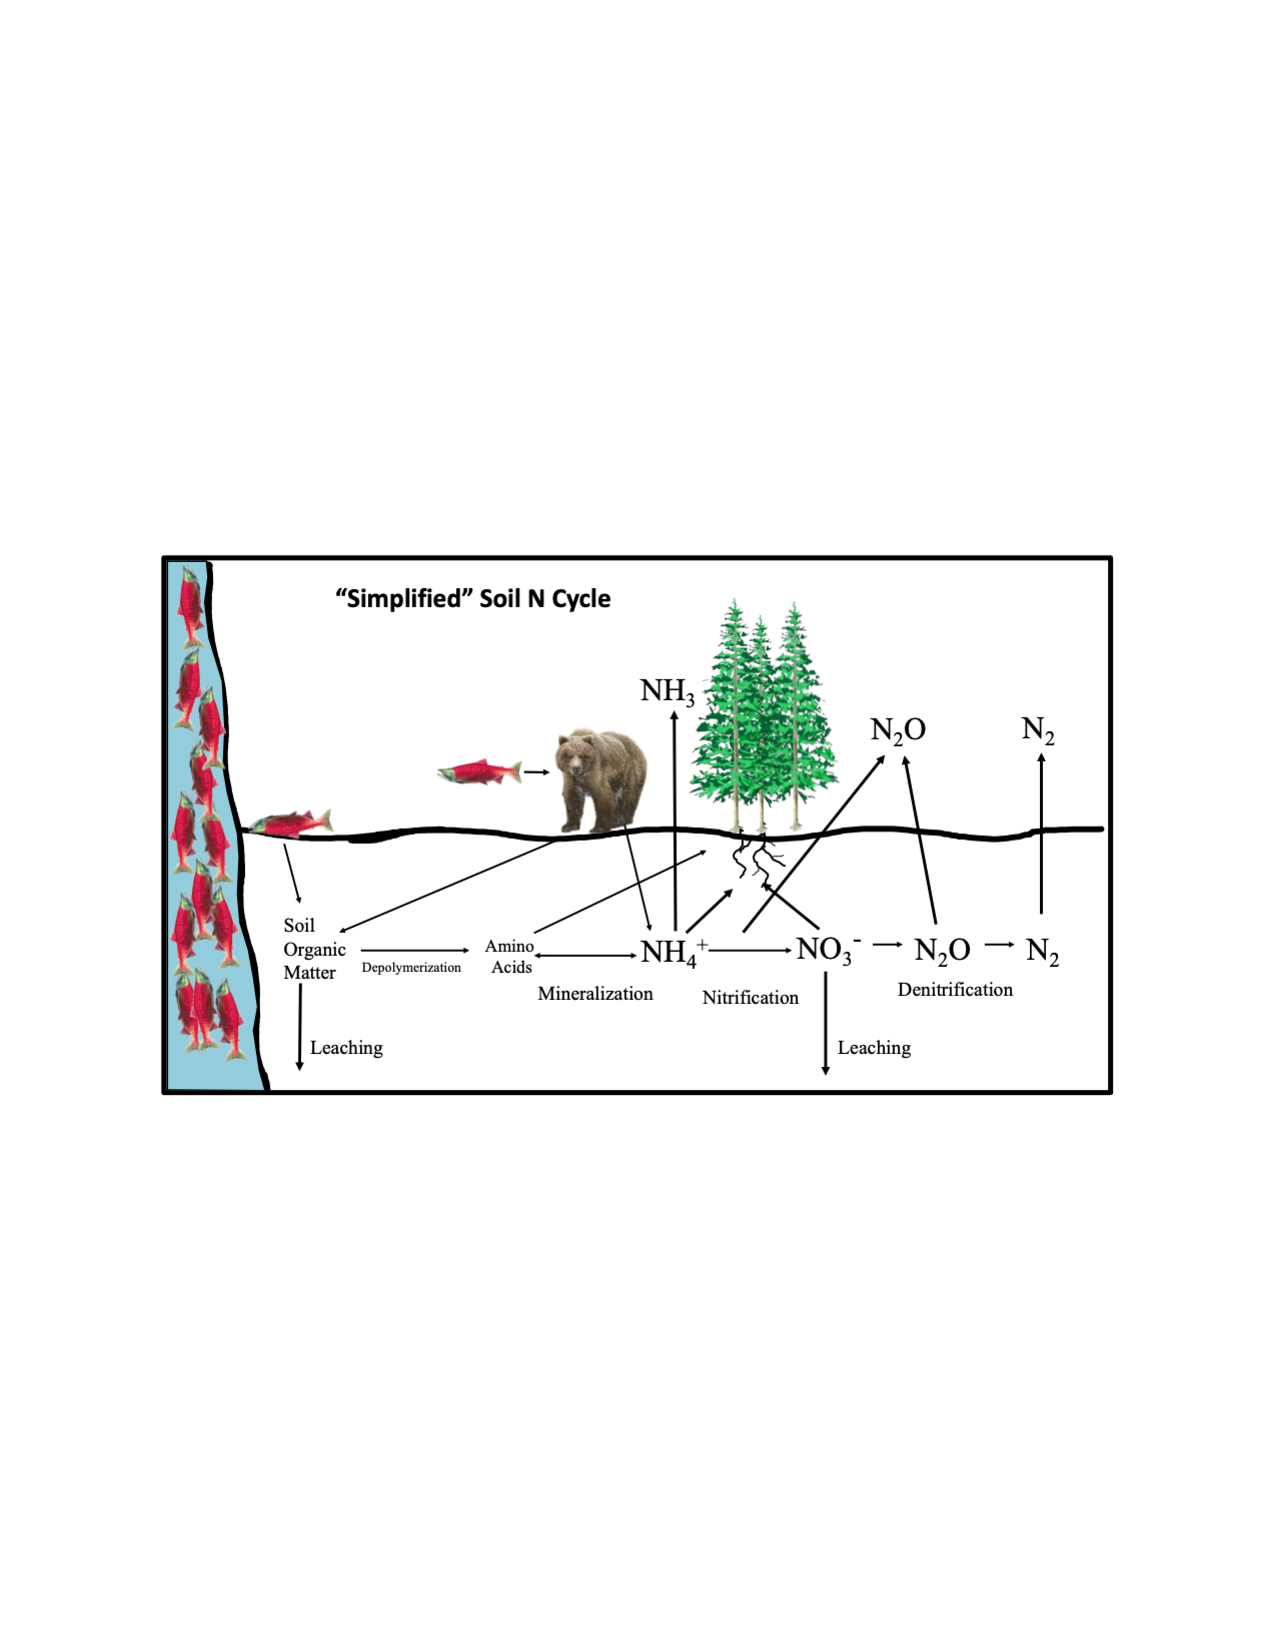
\includegraphics{figure/fig1.1.pdf}
  \caption{Nitrogen pathways in soil}
  \label{fig:npathways}
\end{figure}
\newline Experiments examining the contributions of MDN are often
limited by short timescales, and relatively few experiments investigate
changes in plant-available soil N pools important to plant nutrient
uptake and growth (Collins et al.,
\protect\hyperlink{ref-Collins2015}{2015}). Studies examining spatial
and temporal impacts of salmon on soil inorganic N have identified
highly localized responses (effects only observed \textless{} 30 cm from
carcasses) where soil ammonium (NH\textsubscript{4}\textsuperscript{+})
and nitrate (NO\textsubscript{3}\textsuperscript{-}) increase for weeks
to months (Drake, Naiman, \& Bechtold,
\protect\hyperlink{ref-Drake2006}{2006}; Gende, Miller, \& Hood,
\protect\hyperlink{ref-Gende2007}{2007}; Holtgrieve, Schindler, \&
Jewett, \protect\hyperlink{ref-Holtgrieve2009}{2009}) and rarely
consider long-term N retention in the system. Experiments typically
examine the contributions of MDN by nutrient addition not nutrient
removal; however, nutrient removal is important for understanding the
effects of lower numbers of salmon returning to coastal watersheds due
to fishing, habitat reduction, and climate change. In addition, previous
research observed a strong effect of watershed slope on
\textsuperscript{15}N/\textsuperscript{14}N in riparian plants and
attributed this to topography concentrating carcasses near streams
(Hocking \& Reynolds, \protect\hyperlink{ref-Hocking2012}{2012}).
However, watershed topography also influences soil water content and N
cycling, which affect N isotopes (HÖgberg,
\protect\hyperlink{ref-Hogberg1998}{1998}) and therefore complicates MDN
assessments.

To resolve the extent to which salmon carcasses contributed MDN to
plant-available N pools and the long-term ecological response to this
subsidy, we present a second study of the 20-year carcass manipulation
experiment described in Quinn et al.
(\protect\hyperlink{ref-Quinn2018}{2018}). While Quinn et al.
(\protect\hyperlink{ref-Quinn2018}{2018}) focused on tree growth before
and after the manipulation, the objective of this work was to determine
whether prolonged enhancement and reduction of salmon subsidies altered
long-term soil N cycling, similar to that documented in forests
receiving N fertilizer additions (Lu et al.,
\protect\hyperlink{ref-Lu2011}{2011}; Prescott, Corbin, \& Parkinson,
\protect\hyperlink{ref-Prescott1992}{1992}; Prescott, Kishchuk, \&
Weetman, \protect\hyperlink{ref-Prescott1995}{1995}). If long-term
changes in N availability due to salmon enhancement or reduction were
observed, compensatory nutrient subsidies may be valuable for
maintaining critical ecosystem functions in riparian areas with reduced
salmon returns. If not, then the addition of nutrients as a management
response to low salmon returns may have unintended negative consequences
(sensu Compton et al., \protect\hyperlink{ref-Compton2006}{2006}).
Specifically, the importance of MDN to riparian ecosystems was assessed
by 1) evaluating the presence of MDN in soils enhanced and depleted in
salmon carcasses through bulk stable isotope analysis of N, 2)
quantifying the response of plant-available N pools
({[}NH\textsubscript{4}\textsuperscript{+}{]} and
{[}NO\textsubscript{3}\textsuperscript{-}{]}) and their rate of supply
via mineralization and nitrification, 3) considering how fractionation
in soils may impact mixing model results by measuring
\textsuperscript{15}N/\textsuperscript{14}N of
NH\textsubscript{4}\textsuperscript{+} and 4) comparing these results to
the vegetation responses measured by Quinn et al.
(\protect\hyperlink{ref-Quinn2018}{2018}) at the same site. This
research fills key knowledge gaps by examining the long-term legacy of
inorganic N pools, both salmon addition and removal, and considering
site variability that may impact the assumption of biogeochemical
similarity between test and control sites, following a 20-year
manipulation.

\section{Methods}\label{methods}

\subsection{\texorpdfstring{\emph{Site Description and Sample
Collection}}{Site Description and Sample Collection}}\label{site-description-and-sample-collection}

This study was conducted on Hansen Creek, a \textasciitilde{}2 km long,
2\textsuperscript{nd} order tributary to Lake Aleknagik in the Wood
River system of Bristol Bay, AK and uses the same carcass manipulation
described in Quinn et al. (\protect\hyperlink{ref-Quinn2018}{2018}).
Briefly, from 1997-2016 an average of 10,853 sockeye salmon returned to
the stream annually. Overstory vegetation is dominated by white spruce
and paper birch (\emph{Betula papyrifera}), and unlike many other
watersheds in the region, it has a low density of symbiotic N2-fixing
alder (\emph{Alnus spp.}) (Helfield \& Naiman,
\protect\hyperlink{ref-Helfield2002}{2002}). From 1997-2016 the stream
was surveyed daily during the annual sockeye salmon (\emph{Oncorhynchus
nerka}) run and all dead salmon were removed from the creek and the
river right bank to a distance of about 5 m and tossed onto the river
left bank. To avoid double counting carcasses on the river left bank,
carcasses naturally occurring on the river left bank were also relocated
to a distance of about 5 m, thus all carcasses (with the exception of
those moved by wildlife, see Quinn et al.
(\protect\hyperlink{ref-Quinn2018}{2018})) were located between 3 -- 6 m
on the river left bank. Therefore, the right side of the stream
experienced a reduction in carcass density (depletion) while the left
bank received an increase in carcasses (enhancement). Quinn et al.
(2018) calculated that prior to manipulation the both banks averaged
4545.6 kg of salmon annually and after manipulation the river left bank
averaged 13,381 kg of salmon and the river right bank averaged 2,260 kg
of salmon annually, a 9.6-fold difference. Approximately 108,530
individual fish (in many cases partially consumed by bears) were
translocated over the 20-year period representing a total of 267,620 kg
of salmon, 8,028 kg of N and 1,356 kg of phosphorus (P) (Quinn et al.,
\protect\hyperlink{ref-Quinn2018}{2018}). To estimate the mass of
nitrogen added per m\textsuperscript{2} we assumed all salmon were
tossed within 6 m of the creek's edge along the entire 2 km creek, thus
within a 12,000 m\textsuperscript{2} area.

Soil samples were collected from the riparian zone on 13 July, 2017
(prior to arrival of salmon and any carcass manipulation that season)
along nine sets of paired transect sites. Paired transects were used to
control for naturally occurring salmon density. Transects covered the
full 2 km length of the stream and were selected to represent typical
riparian vegetation and high annual carcass abundance. Each transect
included sampling sites at 1, 3, 6, 10, and 20 m from the bank-full
point. Sampling occurred during peak growing season approximately one
week prior to the arrival of the first salmon in the creek. Thus, our
sampling was intended to capture the long-term legacy of MDN
manipulations and specifically avoid short-term pulses following salmon
return that may not represent a system-level change in N availability,
retention, and recycling in soils, and has already been documented in
multiple short-term studies. A 5 cm x 5 cm x 10 cm soil column was taken
for each sample site and the litter layer was removed before storing at
\(4^{\circ}C\) in airtight plastic bags for 48 hours prior to
processing. Nitrogen cycling decreases dramatically with depth, sampling
at this depth includes the O and A horizons where a majority of nitrogen
cycling occurs (Sparks, Soil Science Society of, \& American Society of,
\protect\hyperlink{ref-Sparks1996}{1996}).

\subsection{\texorpdfstring{\emph{Soil nitrogen concentrations and
transformations}}{Soil nitrogen concentrations and transformations}}\label{soil-nitrogen-concentrations-and-transformations}

Soil {[}NH\textsubscript{4}\textsuperscript{+}{]},
{[}NO\textsubscript{3}\textsuperscript{-}{]}, and N transformations were
measured according to Holtgrieve et al.
(\protect\hyperlink{ref-Holtgrieve2009}{2009}). Briefly, we extracted 10
to 12 g of field-moist sieved (\textless{} 2 mm) soil with 100 mL of 2 M
potassium chloride (KCl) by shaking for 60 s, followed by settling for
24 hours prior to filtration through pre-leached Whatman \#1 filter
papers. Approximately 8 mL of filtered extracts were frozen and later
analyzed colorimetrically for
{[}NH\textsubscript{4}\textsuperscript{+}{]} and
{[}NO\textsubscript{3}\textsuperscript{-}{]} with an Auto-Analyzer 500
Model (Perstorp Analytical Co, Analytical Service Station, Seattle, WA,
USA). The remaining extract was frozen prior to stable isotope analyses
(see below). To estimate inorganic N transformation rates, a second 10
to 12 g soil subsample was incubated aerobically in the dark for 15 d at
\(20^{\circ}C\) prior to extraction, filtration, and analysis as above.
Net mineralization was calculated as the sum of the change in
{[}NH\textsubscript{4}\textsuperscript{+}{]} and
{[}NO\textsubscript{3}\textsuperscript{-}{]} divided by the incubation
duration, and net nitrification was calculated as the change in
{[}NO\textsubscript{3}\textsuperscript{-}{]} over the incubation
duration and represents the conversion of
NH\textsubscript{4}\textsuperscript{+} to
NO\textsubscript{3}\textsuperscript{-} ({\textbf{???}}).
{[}N\textsubscript{org}{]} was calculated by taking total soil N
concentration, {[}N\textsubscript{tot}{]} determined by elemental
analysis (see below) and subtracting
{[}NH\textsubscript{4}\textsuperscript{+}{]} and
{[}NO\textsubscript{3}\textsuperscript{-}{]}. All soil N values were
corrected for gravimetric soil water content (g H2O/g dry soil)
determined by drying 50 to 100 g of field-moist soil at \(105^{\circ}C\)
for 48 h ({\textbf{???}}).

\subsection{\texorpdfstring{\emph{Stable isotope
analysis}}{Stable isotope analysis}}\label{stable-isotope-analysis}

Fresh soil was freeze dried for 48 h and ground into a uniform powder
(\textless{} 212 \(\mu\)m) using a ball mill prior to analysis for
nitrogen (\textsuperscript{15}N/\textsuperscript{14}N) and carbon
(\textsuperscript{13}C/\textsuperscript{12}C) stable isotope ratios at
the University of Washington's IsoLab using a Costech Elemental
Analyzer, Conflo III MAT253 for continuous flow-based measurements. This
procedure also provided total carbon and nitrogen concentrations,
{[}C\textsubscript{tot}{]} and {[}N\textsubscript{tot}{]}, and percent C
and N, of the soil samples. Data are reported using standard delta
notation, which describes the per mil deviation in the ratio of heavy to
light isotope relative to accepted international standards, in this case
air and Vienna Pee Dee Belemite (VPDB) for N and C respectively
({\textbf{???}}).

For \textsuperscript{15}N/\textsuperscript{14}N stable isotope analysis
of NH\textsubscript{4}\textsuperscript{+} and
NO\textsubscript{3}\textsuperscript{-}, KCl extracts were placed in
Erlenmeyer flasks for diffusion using modified methods from Sigman et
al. (\protect\hyperlink{ref-Sigman1997}{1997}) and Holmes, McClelland,
Sigman, Fry, \& Peterson (\protect\hyperlink{ref-Holmes1998}{1998}). To
retrieve NH4+ as gaseous NH3, 300 mg of MgO and an acid trap (1 cm glass
fiber filter treated with KHSO\textsubscript{4} and sealed in Teflon)
were added to each flask, immediately stoppered, sealed with parafilm,
and shaken for six days prior to removal of acid traps to a desiccator
for 3 to 4 days. The same extracts were then shaken uncovered for one
day to remove any remaining NH\textsubscript{4}\textsuperscript{+}. To
retrieve NO\textsubscript{3}\textsuperscript{-} as NH\textsubscript{3},
another 300 mg of MgO were added to each extract and immediately
followed with 75 mg of Devarda's alloy and an acid trap, then processed
as above. Samples were run in four separate batches, for each batch
three blanks (KCl with no soil extract) and three reference standards,
NH\textsubscript{4}Cl and KNO\textsubscript{3} with known
\textsuperscript{15}N/\textsuperscript{14}N, were also run. Batch blanks
showed quantifiable N from the KCl; therefore, a two-source mixing model
correction was applied to both samples and reference standards using
\eqref{eq:blank}:
\begin{equation} 
  \delta^{15}N_{blank corrected} =   \frac{\delta^{15}N_{measured}*(N_{blank,x} + N_{extracted}) - (\delta^{15}N_{blank,x}*N_{blank,x})}{N_{extracted}}
  \label{eq:blank}
\end{equation}
Where \emph{x} represents an individual batch,
\emph{N\textsubscript{blank,x}} is the average measured mass (µg) of
nitrogen in a blank for a given batch, and \(\delta^{15}N_{blank,x}\) is
the average measured \(\delta^{15}N\) of blanks for a given batch.
\(\delta^{15}N_{measured}\) is the \(\delta^{15}N\) value for a given
sample, and \emph{N\textsubscript{extracted}} is the mass of nitrogen
(µg) measured in the sample. A standard correction was then applied to
the blank corrected measurements with \eqref{eq:stand}:
\begin{equation} 
  \delta^{15}N_{corrected} =   \delta^{15}N_{blank,corrected}-(Standard_{measured,x} - Standard_{true})
  \label{eq:stand}
\end{equation}
Where \emph{Standard\textsubscript{measured,x}} is the average measured
value of the standard for a given batch. All reported
\(\delta^{15}N-NH_4^+\) and NO\textsubscript{3}\textsuperscript{-}
values are expressed as the \(\delta^{15}N_{corrected}\), where a blank
and standard correction has been applied. The internal standard of the
\(\delta^{15}N\) of NO\textsubscript{3}\textsuperscript{-} had a -23.6
to 9.6‰ deviation from its true value, indicating a significant
methodological issue. Given there was not enough sample to refine these
methods and the potential for standard corrections of this magnitude to
be misleading, \(\delta^{15}N\) of
NO\textsubscript{3}\textsuperscript{-} data are not reported here.

C:N ratio, percent nitrification, and \%C were also calculated to
evaluate N availability and retention across the sites. C:N ratios were
calculated on a mass basis Percent nitrification was calculated as
\eqref{eq:nit}:
\begin{equation} 
 Percent Nitrification =100 * Net Nitrification / Net Mineralization 
  \label{eq:nit}
\end{equation}
\subsection{\texorpdfstring{\emph{Statistical
analyses}}{Statistical analyses}}\label{statistical-analyses}

We used multi-model selection procedures via Akaike's information
criterion (AIC) to identify how salmon carcass treatment governed a
suite of response variables using the stats v3 and lme4 packages in R.
These response variables were: \(\delta^{15}N\) and \(\delta^{13}C\) of
bulk soil, \(\delta^{15}N\) of NH\textsubscript{4}\textsuperscript{+},
{[}NH\textsubscript{4}\textsuperscript{+}{]} and
{[}NO\textsubscript{3}\textsuperscript{-}{]}, net mineralization and net
nitrification, {[}N\textsubscript{org}{]}, gravimetric water content
(GW), and C:N. For all response variables, candidate models Table
\ref{tab:candmod1} included bank (left vs.~right) and distance from
river's edge. A linear and quadratic interaction structure for bank and
distance were fit for each response variable and these interaction terms
allowed the effect of distance to vary by bank and the effect of bank to
vary by distance. A log\textsubscript{e} transformation was used for the
distance. GW was considered as a covariate for all response variables,
soil {[}NH\textsubscript{4}\textsuperscript{+}{]} was considered as a
covariate for net nitrification, and soil {[}N\textsubscript{org}{]} was
considered as a covariate for net mineralization, given
{[}N\textsubscript{org}{]} and
{[}NH\textsubscript{4}\textsuperscript{+}{]} function as the substrate
for mineralization and nitrification respectively.
{[}N\textsubscript{tot}{]} was considered as a covariate for
\(\delta^{15}N\) and \(\delta^{13}C\) of bulk soil, and for
\(\delta^{15}N\) of NH\textsubscript{4}\textsuperscript{+}. The best
model was selected from the candidate model set using AIC for each
response variable.

\textbf{Table} \ref{tab:candmod1}: The candidate model set tested for
each response variable using AIC analysis where \{*\} denotes models
used for all response variables, additional models were used for net
mineralization and net nitrification where substrate represents organic
nitrogen concentration and NH\textsubscript{4}\textsuperscript{+}
concentration, respectively. For \(\delta^{15}N\) data, GW was not
tested as a covariate and total mass of N was tested instead. The four
tested hypotheses are 1) bank effect, 2) distance effect, 3) bank and
distance effect (salmon effect), and 4) no effect of bank and distance.
Response variables include: \(\delta^{15}N\) and \(\delta^{13}C\) of
bulk soil, \(\delta^{15}N\) of NH\textsubscript{4}\textsuperscript{+},
{[}NH\textsubscript{4}\textsuperscript{+}{]} and
{[}NO\textsubscript{3}\textsuperscript{-}{]}, net mineralization and net
nitrification, {[}N\textsubscript{org}{]}, gravimetric water content
(GW), and C:N.

\begingroup\fontsize{6}{8}\selectfont
\begin{longtable}[t]{lr}
\caption{\label{tab:candmod1}The candidate model set tested for each response variable using AIC analysis}\\
\toprule
Candidate Model Set & Hypothesis\\
\midrule
*Response Variable = bank + ε & 1\\
*Response Variable = bank + GW + ε & 1\\
*Response Variable = ln(distance) + GW + ε & 1\\
*Response Variable = ln(distance) + ε & 1\\
*Response Variable = bank + ln(distance) + bank:ln(distance) + ln(distance)2:bank + GW + ε & 2\\
\addlinespace
*Response Variable = bank + ln(distance) + bank:ln(distance) + ε & 1\\
*Response Variable = bank + ln(distance) + bank:ln(distance) + GW + ε & 1\\
*Response Variable = bank + ln(distance) + bank:ln(distance) + ln(distance)2:bank + ε & 2\\
*Response Variable = bank + ln(distance) + bank+ ε & 1\\
*Response Variable = bank + ln(distance) + bank + GW+ ε & 1\\
\addlinespace
*Response Variable = GW + ε & 3\\
Response Variable = bank + substrate + ε & 1\\
Response Variable = ln(distance) + substrate + ε & 1\\
Response Variable = bank + GW + substrate + ε & 1\\
Response Variable = bank + ln(distance) + bank:ln(distance) + GW + substrate + ε & 2\\
\addlinespace
Response Variable = bank + ln(distacne) + bank:ln(distance) + substrate + ε & 1\\
Response Variable = bank + ln(distance) + bank:ln(distance) + GW + substrate + ε & 2\\
Response Variable = bank + ln(distance) + bank:ln(distance) + ln(distance)2:bank + GW+ substrate + ε & 2\\
Response Variable = bank + ln(distance) + bank:ln(distance) + ln(distance)2:bank + substrate + ε & 2\\
Response Variable = bank + ln(distance)  + GW+ substrate + ε & 1\\
\addlinespace
Response Variable = bank + ln(distance)  +  substrate + ε & 1\\
Response Variable = substrate + ε & 3\\
Response Variable = GW + substrate + ε & 3\\
\bottomrule
\end{longtable}
\endgroup{}

Two model parameters -- bank (left vs.~right) and distance from the
stream -- were used to test salmon carcass and site variability impacts
to soil N cycling. Changing the number of salmon carcasses on each bank
was the primary goal of the manipulation; however, the two banks
potentially differ in aspect, soil type, and drainage, which can affect
nutrient cycling and generate a bank effect unrelated to salmon
manipulation (I. Chapin F. Stuart, Matson, Vitousek, \& Chapin,
\protect\hyperlink{ref-Chapin2011}{2011}). Notably, the salmon enhanced
bank has a northwest facing slope within 20 m of the creek edge.
Distance from the stream reflects the magnitude of salmon manipulation
because carcasses were placed primarily 3 -- 6 m from the stream's edge.
Other factors such as vegetation, soil type, and water availability can
also change with distance laterally from the stream edge, though such
changes are expected to be more continuous, rather than focused on the
same 3 -- 6 m band where salmon were placed. These differences in
expected lateral patterns in soil properties due to salmon (focused at 3
-- 6 m) verse other factors (more continuous) provide a means to test
whether salmon significantly altered soil patterns in our experiment.

We inferred that salmon significantly influenced a soil property when
that soil property met the following conditions: (a) the property
differed between the study banks, (b) varied with distance from the
stream edge, and (c) displayed a peak response at 3 - 6 m on the salmon
addition bank. All conditions (a, b, c) are required to infer that
salmon significantly altered the soils on the treatment bank. In
contrast, we inferred that support for only one of these parameters
demonstrates underlying site variability in the system. Effects of
natural site variability on soil properties is also an important
component to test. Control sites are typically assumed to be
biogeochemically similar to carcass sites without validating this
assumption, despite control sites often being located at different
stream reaches or on different streams altogether. For each of the nine
response variables, three competing hypotheses were compared, that the
differences in response variables were due to H1) a bank and/or distance
effect that does not demonstrate a peak response between 3 -- 6 m
indicating site variability not caused by salmon manipulation, H2) a
bank and distance effect as a quadratic interaction with a peak between
3 -- 6 m indicting a response to salmon manipulation or H3) no
difference caused by distance and bank indicating support for the other
covariates tested. These hypotheses were tested by categorizing each
candidate model into one of the three hypotheses (Table
\ref{tab:candmod1}) and considering the hypothesis categorization for
the model with the most support, and any additional competing models
with relative support (\(\Delta\)AIC value of \textless{} 2)
{[}({\textbf{???}})) for each response variable under consideration
(e.g., {[}NH4+{]}, {[}NO3-{]}, \(\delta^{15}N\), etc.). If models showed
support for H2, the effect of salmon was confirmed by examining whether
the response variable peaked at the salmon enhanced bank between 3 -- 6
m. If this did not occur, the response is due to site variability and
not salmon.

\section{Results}\label{results}

Bulk soil stable isotope analysis indicated that salmon carcasses
enriched the N isotope pools (Table 1). \(\delta^{15}N\) values peaked
between 3 and 6 m from the stream edge, which was the distance salmon
were typically relocated to during the experiment and declined at
distances greater than 6 m. Maximum \(\delta^{15}N\) of bulk soils was
11.8‰ for the salmon enhanced bank and 11.6‰ for the salmon depleted
bank and no observations exceeded the sockeye salmon end-member value of
12.6‰ (Figure 2a). \(\delta^{13}C\) was more enriched at greater
distances from the bank and on average was highest at 20 m (Figure 2b).
\(\delta^{13}C\) was primarily governed by distance, with some evidence
{[}N\textsubscript{tot}{]} and bank also had an effect (
\ref{tab:suppmod1}).

\textbf{Table} \ref{tab:suppmod1}: Competing models with relative
support (ΔAIC \textless{} 2) using AIC analysis for each response
variable, where the most parsimonious models with the most support are
shown in bold. Reported are ΔAIC and the hypothesis supported by each
model: H1 is a bank effect not caused by salmon manipulation, H2 is a
distance effect not caused by salmon manipulation, H3 is both a bank and
distance effect indicating a response to salmon manipulation, and H4
indicates support for the other covariates tested.

\begingroup\fontsize{8}{10}\selectfont
\begin{longtable}[t]{lrrl}
\caption{\label{tab:suppmod1}Competing models with relative support (ΔAIC < 2) using AIC analysis for each response variable}\\
\toprule
Response Variable & Model Hypothesis & ΔAIC & Covariates Included in Models with Relative Support\\
\midrule
Bulk δ15N & 2 & 0.00 & Bank, ln(Distance), Bank:ln(Distance), Bank:ln(Distance)2\\
 & 2 & 0.41 & Bank, ln(Distance), Bank:ln(Distance), Bank:ln(Distance)2, [Ntot]\\
Bulk δ13C & 1 & 0.00 & ln(Distance)\\
 & 1 & 0.22 & Bank, ln(Distance)\\
 & 1 & 0.62 & ln(Distance), [Ntot]\\
\addlinespace
 & 1 & 1.23 & Bank, ln(Distance), [Ntot]\\
δ15N of NH4+ & 2 & 0.00 & Bank, ln(Distance), Bank:ln(Distance), Bank:ln(Distance)2\\
{}[NH4+] & 1 & 0.00 & Bank, ln(Distance)\\
 & 1 & 0.69 & Bank, ln(Distance), Bank:ln(Distance)\\
 & 1 & 0.69 & Bank\\
\addlinespace
 & 1 & 0.95 & Bank, GW\\
 & 1 & 1.10 & Bank, ln(Distance), GW\\
 & NA & NA & \\
 & 1 & 1.87 & Bank, ln(Distance), Bank:ln(Distance), GW\\
{}[NO3-] & 1 & 0.00 & Bank, GW\\
\addlinespace
 & 1 & 1.72 & Bank, ln(Distance), GW\\
 & 2 & 1.87 & Bank, ln(Distance), Bank:ln(Distance), Bank:ln(Distance)2, GW\\
Net Mineralization & 3 & 0.00 & {}[NOrg]\\
 & 3 & 0.61 & GW, [NOrg]\\
 & 1 & 0.74 & Bank, [NOrg]\\
\addlinespace
 & 1 & 1.61 & Bank, GW, [NOrg]\\
Net Nitrification & 3 & 0.00 & {}[NH4+], GW\\
 & NA & NA & \\
 & 1 & 1.02 & Bank, [NH4+], GW\\
{}[NOrg] & 1 & 0.00 & ln(Distance), GW\\
\addlinespace
 & 1 & 0.22 & Bank, ln(Distance), Bank:ln(Distance), GW\\
 & 2 & 0.33 & Bank, ln(Distance), Bank:ln(Distance), Bank:ln(Distance)2, GW\\
 & 1 & 1.94 & Bank, ln(Distance), GW\\
Gravimetric Water Content (GW) & 1 & 0.00 & ln(Distance), Bank\\
 & 1 & 1.00 & ln(Distance)\\
\addlinespace
 & 1 & 1.80 & Bank, ln(Distance), Bank:ln(Distance)\\
\bottomrule
\end{longtable}
\endgroup{}

Salmon carcass manipulation also enriched \(\delta^{15}N\) of soil
NH\textsubscript{4}\textsuperscript{+}. Stable isotope values were
enriched at 3 m from the stream edge on the salmon enhanced bank, and
declined at distances \textgreater{} 3 m. On the salmon depleted bank,
\(\delta^{15}N\) of soil NH\textsubscript{4}\textsuperscript{+} was most
enriched at 1 m and declined with distance (Figure
@ref(fig:modsupp1.2)C). The only model with support contained a
quadratic interaction of distance and bank, which provides strong
evidence that \(\delta^{15}N\) of NH4+ was affected by salmon (Table
\ref{tab:suppmod1}). In contrast to bulk soil N, \(\delta^{15}N\) values
of NH\textsubscript{4}\textsuperscript{+} exceeded the salmon endmember
of 12.6‰ for 23\% of all observations (n=21).

Inorganic nitrogen concentrations were primarily governed by bank and GW
(Table \ref{tab:suppmod1}). The salmon enhanced bank had a higher mean
{[}NH\textsubscript{4}\textsuperscript{+}{]} and
{[}NO\textsubscript{3}\textsuperscript{-}{]} compared to the salmon
depleted bank (Figure 2d, e). The most supported models for both
{[}NH\textsubscript{4}\textsuperscript{+}{]} and
{[}NO\textsubscript{3}\textsuperscript{-}{]} showed evidence for H1,
that observed differences were not caused by salmon. For
{[}NH\textsubscript{4}\textsuperscript{+}{]} there was substantial model
uncertainty, with six competing models receiving relative support (ΔAIC
\textless{} 2) (Table \ref{tab:suppmod1}) but none of the competing
models supported a salmon effect. Two competing models for
{[}NO\textsubscript{3}\textsuperscript{-}{]} supported a site
variability effect and one competing model supported a salmon effect
(Tabe \ref{tab:suppmod1}) and all three contained gravimetric water
content as a covariate. This indicates
{[}NH\textsubscript{4}\textsuperscript{+}{]} was driven by site factors
unrelated to salmon while {[}NO\textsubscript{3}\textsuperscript{-}{]}
was driven by gravimetric water content and with some support for salmon
enhancement.

\textbf{Figure} \ref{fig:modIsotope}: Data (closed circles) and
predicted values (open circles) for the model with the most support
(Table \ref{tab:suppmod1}) for soil organic \(\delta^{15}N\) and
\(\delta^{13}C\), \(\delta^{15}N\) of
NH\textsubscript{4}\textsuperscript{+}, and C:N for both the
salmon-enhanced and the salmondepleted banks of Hansen Creek at 1, 3, 6,
10, and 20 m from the edge of the creek bed with 95\% confidence
intervals (dashed line) for predicted values. Blue (a and c) denotes
measures of marine-derived nitrogen, and green (b and d) denotes site
variable factors.\newline
\begin{figure}[h]
  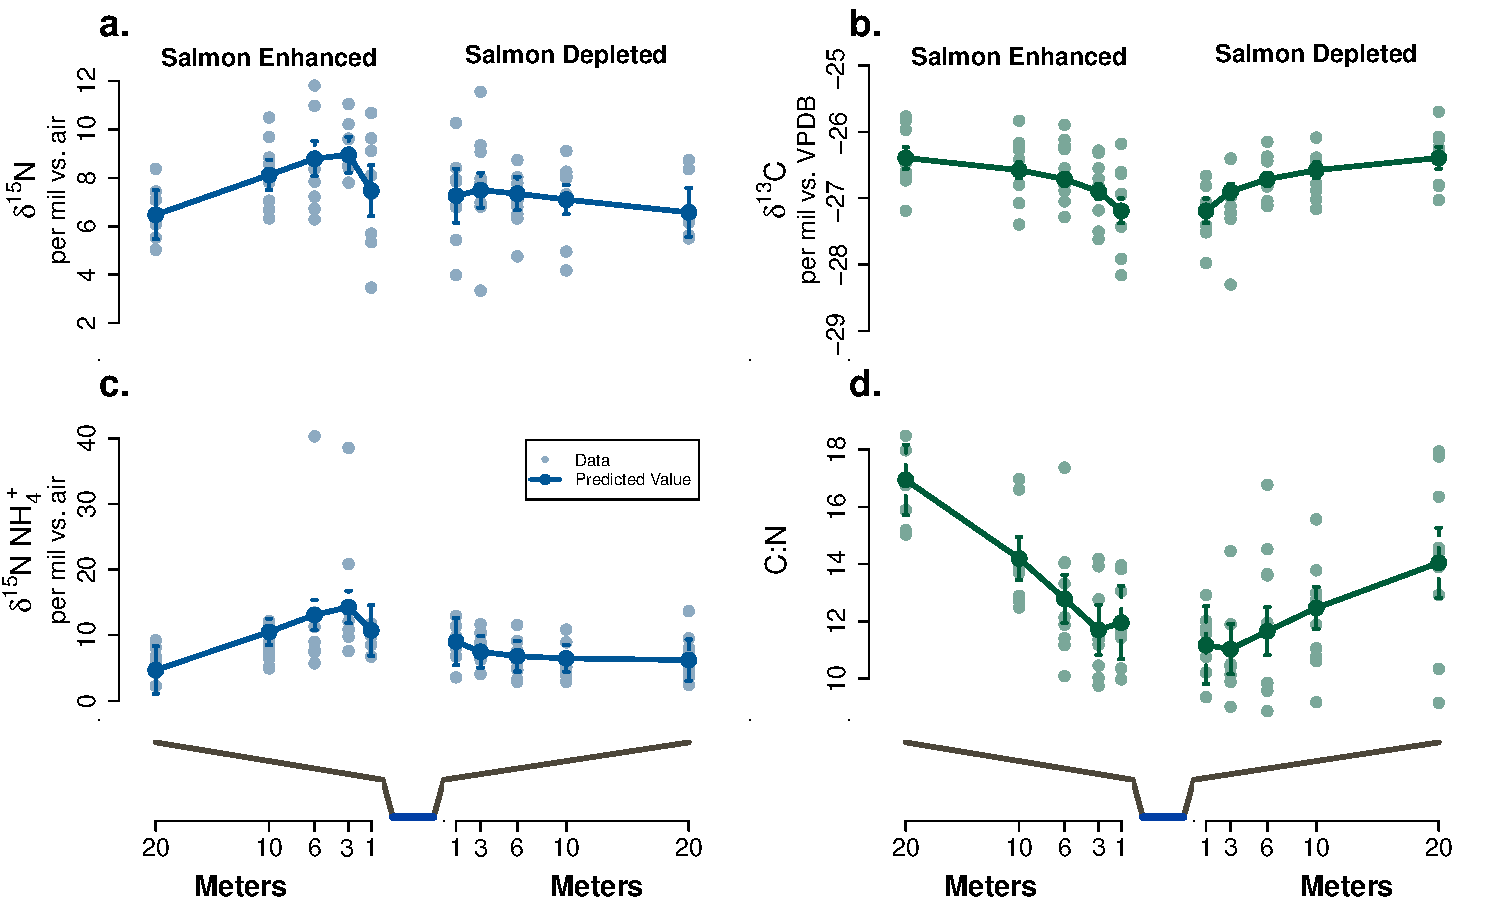
\includegraphics[width=0.85\textwidth]{figure/Figure2_Feddernetal.pdf}
  \caption{Data and predicted values for the model with the most support: Stable Isotopes}
  \label{fig:modIsotope}
\end{figure}
\newline

Nitrogen transformation rates were unaffected by salmon carcass
manipulation. Both net nitrification and net mineralization models with
relative support contained N substrate ({[}NH4+{]} and {[}Norg{]}
respectively), and the models with the most support did not include
distance or bank. Net mineralization had some model uncertainty, with
four models receiving relative support; however, all of the competing
models supported either H1 or H3 with no support for a salmon effect.
{[}Norg{]} was the only covariate included in all of the competing
models, indicating {[}Norg{]} was the most important covariate tested
for determining net mineralization. Net nitrification had greater model
certainty and both models that received relative support contained
{[}NH4+{]} and gravimetric water content. Similar to net mineralization,
these models supported H1 and H3 with no support for H2, the salmon
effect, though net nitrification was slightly higher on average between
3 -- 6 m on the salmon enhanced bank (Table 1). Overall, these results
demonstrated the manipulation of salmon carcasses did not have clearly
detectable effects on N transformation rates.

\textbf{Figure} \ref{fig:modConc}: Data (closed circles) and predicted
values (open circles) for the model with the most support (Table
\ref{tab:suppmod1}) for NH\textsubscript{4}\textsuperscript{+} and
NO\textsubscript{3}\textsuperscript{-}, net mineralization and
nitrification, {[}N\textsubscript{org}{]}, and gravimetric water content
for both the salmon-enhanced and the salmon-depleted banks of Hansen
Creek at 1, 3, 6, 10, and 20 m from the edge of the creek bed with 95\%
confidence intervals (dashed line) for predicted values. Red (a, b, c,
d) denotes measures of soil productivity, and green (e and f) denotes
site variable factors.\newline 
\begin{figure}[h]
  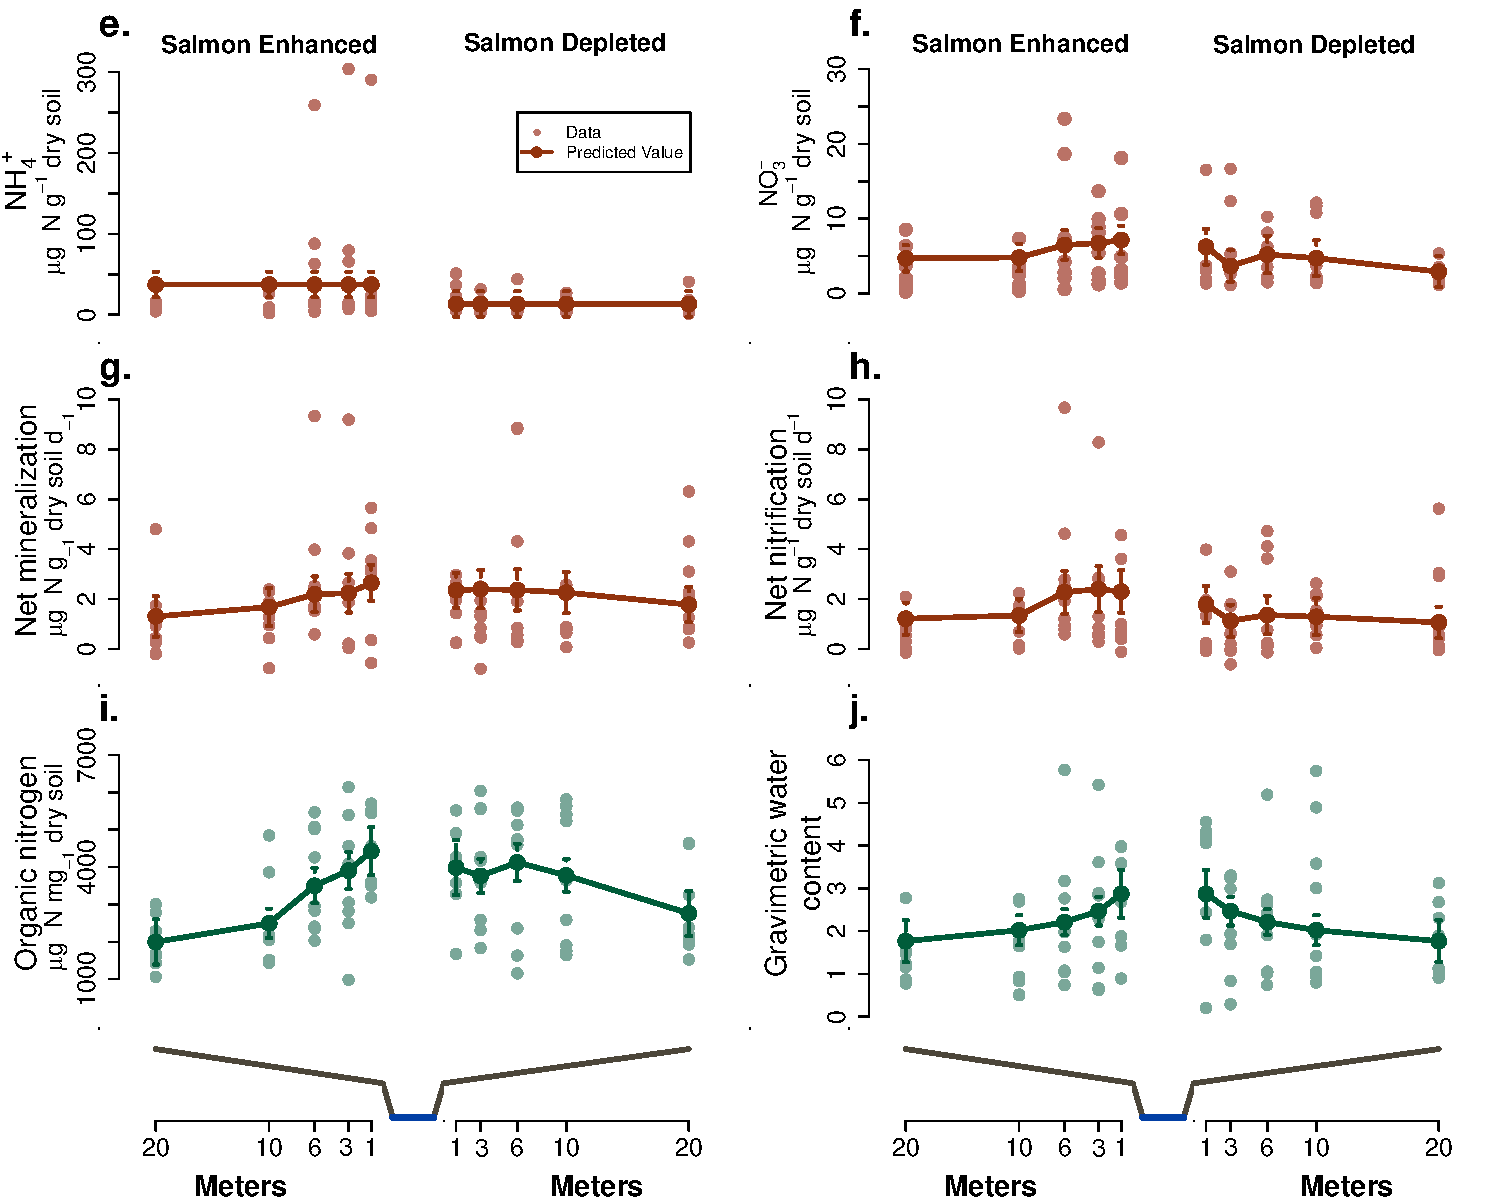
\includegraphics[width=0.85\textwidth]{figure/Figure3_Feddernetal.pdf}
  \caption{Data and predicted values for the model with the most support: Concentrations and Transformations}
  \label{fig:modConc}
\end{figure}
\newline 

Both {[}Norg{]} and GW indicated there are site differences caused by
distance and bank unrelated to salmon carcass manipulation. On average
{[}Norg{]} was higher on the salmon depleted bank than the salmon
enhanced bank. There was model support of H1 for both GW and {[}Norg{]},
indicating these variables decrease with distance (Table 1, Figure 2 h,
i). While there was some evidence that there was both a distance and
bank effect on GW, it was not caused by salmon as the salmon enhanced
bank does not show a peak GW at 3 - 6 m from the stream, which was where
there was the highest observed isotopic enrichment and expected MDN.
However, one competing model for {[}Norg{]} did support H2, indicating
site factors and salmon may both affect {[}Norg{]}. However, the mean
{[}Norg{]} for the salmon enhanced bank was 18.42 mg/g and 18.97 mg/g
for the salmon depleted bank indicating salmon decrease {[}Norg{]}, if
they affect it at all. C:N, percent nitrification, and percent carbon
indicate relatively high nitrogen availability across sampling sites in
the Hansen Creek system. Mean percent carbon was 24.2 and 24.9 on the
enhanced and depleted banks respectively (S3). Soil C:N of bulk isotopes
was less than 20 for all sites, with a mean of 15.8 (enhanced) and 14.2
(depleted). These values are well below the critical microbial C:N
threshold of 29, demonstrating N is more available to meet microbial
metabolic demands relative to C (Figure 2j). In contrast, percent
nitrification was relatively high with a mean of 64\% and 62\% on the
enhanced and depleted banks (S3).

\chapter{Mathematics and Science}\label{math-sci}

\section{Math}\label{math}

\TeX~is the best way to typeset mathematics. Donald Knuth designed
\TeX~when he got frustrated at how long it was taking the typesetters to
finish his book, which contained a lot of mathematics. One nice feature
of \emph{R Markdown} is its ability to read LaTeX code directly.

If you are doing a thesis that will involve lots of math, you will want
to read the following section which has been commented out. If you're
not going to use math, skip over or delete this next commented section.

\section{Chemistry 101: Symbols}\label{chemistry-101-symbols}

Chemical formulas will look best if they are not italicized. Get around
math mode's automatic italicizing in LaTeX by using the argument
\texttt{\$\textbackslash{}mathrm\{formula\ here\}\$}, with your formula
inside the curly brackets. (Notice the use of the backticks here which
enclose text that acts as code.)

So, \(\mathrm{Fe_2^{2+}Cr_2O_4}\) is written
\texttt{\$\textbackslash{}mathrm\{Fe\_2\^{}\{2+\}Cr\_2O\_4\}\$}.

\noindent Exponent or Superscript: \(\mathrm{O^-}\)

\noindent Subscript: \(\mathrm{CH_4}\)

To stack numbers or letters as in \(\mathrm{Fe_2^{2+}}\), the subscript
is defined first, and then the superscript is defined.

\noindent Bullet: CuCl \(\bullet\) \(\mathrm{7H_{2}O}\)

\noindent Delta: \(\Delta\)

\noindent Reaction Arrows: \(\longrightarrow\) or
\(\xrightarrow{solution}\)

\noindent Resonance Arrows: \(\leftrightarrow\)

\noindent Reversible Reaction Arrows: \(\rightleftharpoons\)

\subsection{Typesetting reactions}\label{typesetting-reactions}

You may wish to put your reaction in an equation environment, which
means that LaTeX will place the reaction where it fits and will number
the equations for you.
\begin{equation}
  \mathrm{C_6H_{12}O_6  + 6O_2} \longrightarrow \mathrm{6CO_2 + 6H_2O}
  \label{eq:reaction}
\end{equation}
We can reference this combustion of glucose reaction via Equation
\eqref{eq:reaction}.

\subsection{Other examples of
reactions}\label{other-examples-of-reactions}

\(\mathrm{NH_4Cl_{(s)}}\) \(\rightleftharpoons\)
\(\mathrm{NH_{3(g)}+HCl_{(g)}}\)

\noindent \(\mathrm{MeCH_2Br + Mg}\) \(\xrightarrow[below]{above}\)
\(\mathrm{MeCH_2\bullet Mg \bullet Br}\)

\section{Physics}\label{physics}

Many of the symbols you will need can be found on the math page
\url{http://web.reed.edu/cis/help/latex/math.html} and the Comprehensive
LaTeX Symbol Guide
(\url{http://mirror.utexas.edu/ctan/info/symbols/comprehensive/symbols-letter.pdf}).

\section{Biology}\label{biology}

You will probably find the resources at
\url{http://www.lecb.ncifcrf.gov/~toms/latex.html} helpful, particularly
the links to bsts for various journals. You may also be interested in
TeXShade for nucleotide typesetting
(\url{http://homepages.uni-tuebingen.de/beitz/txe.html}). Be sure to
read the proceeding chapter on graphics and tables.

\hypertarget{ref-labels}{\chapter{Tables, Graphics, References, and
Labels}\label{ref-labels}}

\hypertarget{tables}{\section{Tables}\label{tables}}

By far the easiest way to present tables in your thesis is to store the
contents of the table in a CSV or Excel file, then read that file in to
your R Markdown document as a data frame. Then you can style the table
with the \texttt{kable} function, or functions in the
\href{https://cran.r-project.org/web/packages/kableExtra/index.html}{kableExtra}
pacakge.

In addition to the tables that can be automatically generated from a
data frame in \textbf{R} that you saw in {[}R Markdown Basics{]} using
the \texttt{kable} function, you can also create tables using
\emph{pandoc}. (More information is available at
\url{http://pandoc.org/README.html\#tables}.) This might be useful if
you don't have values specifically stored in \textbf{R}, but you'd like
to display them in table form. Below is an example. Pay careful
attention to the alignment in the table and hyphens to create the rows
and columns. Generally I don't recommend this approach of typing the
table directly into your R Markdown document.
\begin{longtable}[]{@{}ccc@{}}
\caption{\label{tab:inher} Correlation of Inheritance Factors for Parents
and Child}\tabularnewline
\toprule
\begin{minipage}[b]{0.29\columnwidth}\centering\strut
Factors\strut
\end{minipage} & \begin{minipage}[b]{0.47\columnwidth}\centering\strut
Correlation between Parents \& Child\strut
\end{minipage} & \begin{minipage}[b]{0.16\columnwidth}\centering\strut
Inherited\strut
\end{minipage}\tabularnewline
\midrule
\endfirsthead
\toprule
\begin{minipage}[b]{0.29\columnwidth}\centering\strut
Factors\strut
\end{minipage} & \begin{minipage}[b]{0.47\columnwidth}\centering\strut
Correlation between Parents \& Child\strut
\end{minipage} & \begin{minipage}[b]{0.16\columnwidth}\centering\strut
Inherited\strut
\end{minipage}\tabularnewline
\midrule
\endhead
\begin{minipage}[t]{0.29\columnwidth}\centering\strut
Education\strut
\end{minipage} & \begin{minipage}[t]{0.47\columnwidth}\centering\strut
-0.49\strut
\end{minipage} & \begin{minipage}[t]{0.16\columnwidth}\centering\strut
Yes\strut
\end{minipage}\tabularnewline
\begin{minipage}[t]{0.29\columnwidth}\centering\strut
Socio-Economic Status\strut
\end{minipage} & \begin{minipage}[t]{0.47\columnwidth}\centering\strut
0.28\strut
\end{minipage} & \begin{minipage}[t]{0.16\columnwidth}\centering\strut
Slight\strut
\end{minipage}\tabularnewline
\begin{minipage}[t]{0.29\columnwidth}\centering\strut
Income\strut
\end{minipage} & \begin{minipage}[t]{0.47\columnwidth}\centering\strut
0.08\strut
\end{minipage} & \begin{minipage}[t]{0.16\columnwidth}\centering\strut
No\strut
\end{minipage}\tabularnewline
\begin{minipage}[t]{0.29\columnwidth}\centering\strut
Family Size\strut
\end{minipage} & \begin{minipage}[t]{0.47\columnwidth}\centering\strut
0.18\strut
\end{minipage} & \begin{minipage}[t]{0.16\columnwidth}\centering\strut
Slight\strut
\end{minipage}\tabularnewline
\begin{minipage}[t]{0.29\columnwidth}\centering\strut
Occupational Prestige\strut
\end{minipage} & \begin{minipage}[t]{0.47\columnwidth}\centering\strut
0.21\strut
\end{minipage} & \begin{minipage}[t]{0.16\columnwidth}\centering\strut
Slight\strut
\end{minipage}\tabularnewline
\bottomrule
\end{longtable}
We can also create a link to the table by doing the following: Table
\ref{tab:inher}. If you go back to {[}Loading and exploring data{]} and
look at the \texttt{kable} table, we can create a reference to this max
delays table too: Table \ref{tab:maxdelays}. The addition of the
\texttt{(\textbackslash{}\#tab:inher)} option to the end of the table
caption allows us to then make a reference to Table
\texttt{\textbackslash{}@ref(tab:label)}. Note that this reference could
appear anywhere throughout the document after the table has appeared.

\clearpage

\section{Figures}\label{figures}

If your thesis has a lot of figures, \emph{R Markdown} might behave
better for you than that other word processor. One perk is that it will
automatically number the figures accordingly in each chapter. You'll
also be able to create a label for each figure, add a caption, and then
reference the figure in a way similar to what we saw with tables
earlier. If you label your figures, you can move the figures around and
\emph{R Markdown} will automatically adjust the numbering for you. No
need for you to remember! So that you don't have to get too far into
LaTeX to do this, a couple \textbf{R} functions have been created for
you to assist. You'll see their use below.

In the \textbf{R} chunk below, we will load in a picture stored as
\texttt{uw.png} in our main directory. We then give it the caption of
``UW logo'', the label of ``uwlogo'', and specify that this is a figure.
Make note of the different \textbf{R} chunk options that are given in
the R Markdown file (not shown in the knitted document).
\begin{Shaded}
\begin{Highlighting}[]
\NormalTok{knitr}\OperatorTok{::}\KeywordTok{include_graphics}\NormalTok{(}\DataTypeTok{path =} \StringTok{"figure/uw.png"}\NormalTok{)}
\end{Highlighting}
\end{Shaded}
\begin{figure}

\includegraphics[width=6.25in]{figure/uw} \caption{UW logo}\label{fig:uwlogo}
\end{figure}
Here is a reference to the UW logo: Figure \ref{fig:uwlogo}. Note the
use of the \texttt{fig:} code here. By naming the \textbf{R} chunk that
contains the figure, we can then reference that figure later as done in
the first sentence here. We can also specify the caption for the figure
via the R chunk option \texttt{fig.cap}.

\clearpage 

Below we will investigate how to save the output of an \textbf{R} plot
and label it in a way similar to that done above. Recall the
\texttt{flights} dataset from Chapter \ref{rmd-basics}. (Note that we've
shown a different way to reference a section or chapter here.) We will
next explore a bar graph with the mean flight departure delays by
airline from Portland for 2014. Note also the use of the \texttt{scale}
parameter which is discussed on the next page.
\begin{Shaded}
\begin{Highlighting}[]
\NormalTok{flights }\OperatorTok\StringTok{ }\KeywordTok{group_by}\NormalTok{(carrier) }\OperatorTok
\StringTok{  }\KeywordTok{summarize}\NormalTok{(}\DataTypeTok{mean_dep_delay =} \KeywordTok{mean}\NormalTok{(dep_delay)) }\OperatorTok
\StringTok{  }\KeywordTok{ggplot}\NormalTok{(}\KeywordTok{aes}\NormalTok{(}\DataTypeTok{x =}\NormalTok{ carrier, }\DataTypeTok{y =}\NormalTok{ mean_dep_delay)) }\OperatorTok{+}
\StringTok{  }\KeywordTok{geom_bar}\NormalTok{(}\DataTypeTok{position =} \StringTok{"identity"}\NormalTok{, }\DataTypeTok{stat =} \StringTok{"identity"}\NormalTok{, }\DataTypeTok{fill =} \StringTok{"red"}\NormalTok{)}
\end{Highlighting}
\end{Shaded}
\begin{verbatim}
`summarise()` ungrouping output (override with `.groups` argument)
\end{verbatim}
\begin{figure}
\centering
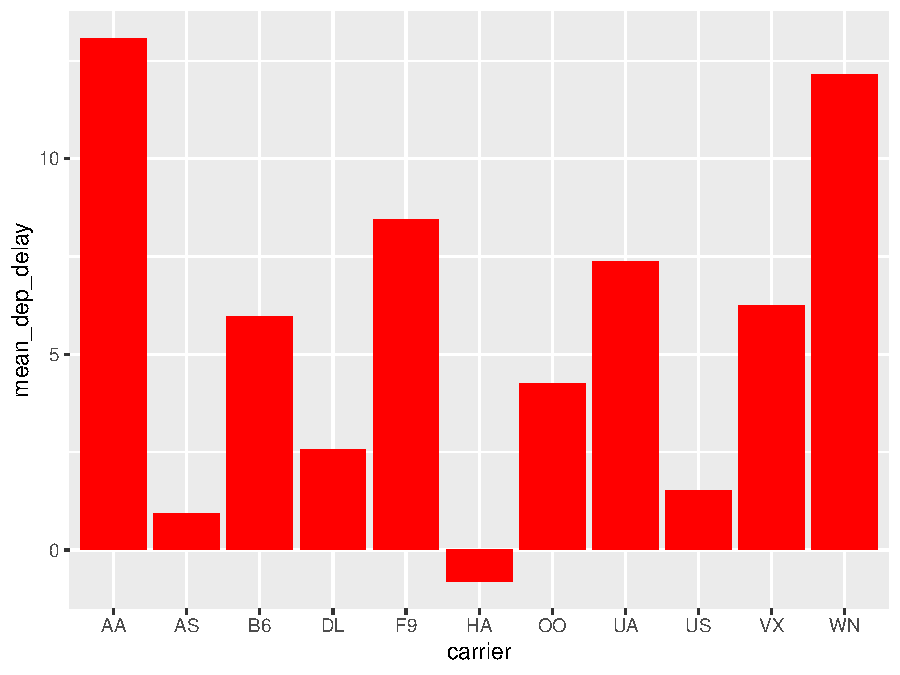
\includegraphics{thesis_files/figure-latex/delaysboxplot-1.pdf}
\caption{\label{fig:delaysboxplot}Mean Delays by Airline}
\end{figure}
Here is a reference to this image: Figure \ref{fig:delaysboxplot}.

A table linking these carrier codes to airline names is available at
\url{https://github.com/ismayc/pnwflights14/blob/master/data/airlines.csv}.

\clearpage

Next, we will explore the use of the \texttt{out.extra} chunk option,
which can be used to shrink or expand an image loaded from a file by
specifying \texttt{"scale=\ "}. Here we use the mathematical graph
stored in the ``subdivision.pdf'' file.
\begin{figure}
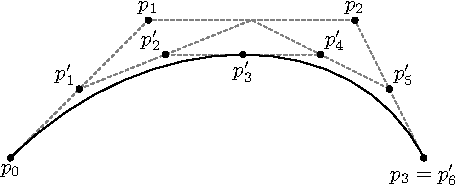
\includegraphics[scale=0.75]{figure/subdivision} \caption{Subdiv. graph}\label{fig:subd}
\end{figure}
Here is a reference to this image: Figure \ref{fig:subd}. Note that
\texttt{echo=FALSE} is specified so that the \textbf{R} code is hidden
in the document.

\textbf{More Figure Stuff}

Lastly, we will explore how to rotate and enlarge figures using the
\texttt{out.extra} chunk option. (Currently this only works in the PDF
version of the book.)
\begin{figure}
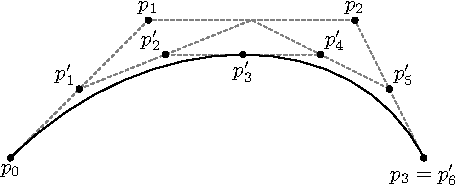
\includegraphics[angle=180, scale=1.1]{figure/subdivision} \caption{A Larger Figure, Flipped Upside Down}\label{fig:subd2}
\end{figure}
As another example, here is a reference: Figure \ref{fig:subd2}.

\section{Footnotes and Endnotes}\label{footnotes-and-endnotes}

You might want to footnote something.\footnote{footnote text} The
footnote will be in a smaller font and placed appropriately. Endnotes
work in much the same way.

\section{Cross-referencing chapters and
sections}\label{cross-referencing-chapters-and-sections}

The
\href{https://bookdown.org/yihui/bookdown/cross-references.html}{bookdown
documentation} is an excellent source for learning how to
cross-reference in a bookdown project such as a huskydown document. Here
we only cover the most common uses for a typical thesis. If you want
something more complex or fancy, please refer to the bookdown
documentation and seek help from the developers of that package.

By default, all of your chapter and section headers will get an
auto-generated ID label For example, e.g., \texttt{\#\ Chapter\ 1} will
have an auto-generated ID \texttt{chapter-1}. Note that the ID label is
all lower case, and has no spaces. If you have any kind of punctuation
in your header, such as a colon (:), it will not appear in the ID label.
Then in your text you can reference chapter one in your Rmd file like
this: `as discussed in Chapter
\texttt{\textbackslash{}@ref(chapter-1)}', which will print as `as
discussed in Chapter 1'

We strongly recommend that you to manually assign ID labels to your
chapter header to make it easy to cross-reference. For example, at the
top of the Rmd file for this chapter, you can see:

\texttt{\#\ Tables,\ Graphics,\ References,\ and\ Labels\ \{\#ref-labels\}}

The \texttt{\{\#ref-labels\}} part of this header is the ID label. It
doesn't show in the output, but is there for us to use for easy
cross-referencing, because it can be short, and we don't need to change
it elsewhere our document when we update the chapter header. We can use
this custom ID label in our Rmd document like this: `as discussed in
Chapter \texttt{\textbackslash{}@ref(ref-labels)}', which will print as
`as discussed in Chapter \ref{ref-labels}'. If you need to show custom
text instead of the chapter number, you use this syntax in your Rmd
document:
\texttt{see\ {[}my\ chapter\ about\ labels{]}(\#ref-labels)\ for\ more\ details}
which will appear as `see \protect\hyperlink{ref-labels}{my chapter
about labels} for more details'

To cross-reference a specific section in the same chapter, we recommend
adding a custom ID label to the section header, and using that to
cross-reference. For example, earlier in this chapter we have a section
on tables and in the Rmd file we see
\texttt{\#\#\ Tables\ \{\#tables\}}. We can cross-reference that in the
text like this `as discussed in the section on
\texttt{{[}tables{]}(\#tables)}' which will appear as `as discussed in
the above section on \protect\hyperlink{tables}{tables}'

To cross-reference a section in a different chapter we can use the ID
label from that section directly. For example, we can write in our Rmd
document
\texttt{as\ discussed\ in\ the\ section\ on\ {[}R\ code\ chunks{]}(\#r-chunks)\ in\ Chapter\ \textbackslash{}@ref(rmd-basics)}
which will appear as `as discussed in the section on
\protect\hyperlink{r-chunks}{R code chunks} in Chapter
\ref{rmd-basics}'.

If you prefer to cross-reference by the section number, we can use
custom ID labels in our Rmd document. For example, to refer to a section
in our first chapter, we can write in the Rmd document:
\texttt{as\ discussed\ in\ section\ \textbackslash{}@ref(r-chunks)\ in\ Chapter\ \textbackslash{}@ref(rmd-basics)}.
This will appear with section and chapter numbers like so: as `as
discussed in section \ref{r-chunks} in Chapter \ref{rmd-basics}'.

\section{Bibliographies}\label{bibliographies}

Of course you will need to cite things, and you will probably accumulate
an armful of sources. There are a variety of tools available for
creating a bibliography database (stored with the .bib extension). In
addition to BibTeX suggested below, you may want to consider using the
free and easy-to-use tool called Zotero. Some Zotero documentation is at
\url{http://libguides.reed.edu/citation/zotero}. In addition, a tutorial
is available from Middlebury College at
\url{http://sites.middlebury.edu/zoteromiddlebury/}.

\emph{R Markdown} uses \emph{pandoc} (\url{http://pandoc.org/}) to build
its bibliographies. One nice caveat of this is that you won't have to do
a second compile to load in references as standard LaTeX requires. To
cite references in your thesis (after creating your bibliography
database), place the reference name inside square brackets and precede
it by the ``at'' symbol. For example, here's a reference to a book about
worrying: ({\textbf{???}}). This \texttt{Molina1994} entry appears in a
file called \texttt{thesis.bib} in the \texttt{bib} folder. This
bibliography database file was created by a program called BibTeX. You
can call this file something else if you like (look at the YAML header
in the main .Rmd file) and, by default, is to placed in the \texttt{bib}
folder.

For more information about BibTeX and bibliographies, see
(\url{http://web.reed.edu/cis/help/latex/index.html})\footnote{({\textbf{???}})}.
There are three pages on this topic: \emph{bibtex} (which talks about
using BibTeX, at \url{http://web.reed.edu/cis/help/latex/bibtex.html}),
\emph{bibtexstyles} (about how to find and use the bibliography style
that best suits your needs, at
\url{http://web.reed.edu/cis/help/latex/bibtexstyles.html}) and
\emph{bibman} (which covers how to make and maintain a bibliography by
hand, without BibTeX, at
\url{http://web.reed.edu/cis/help/latex/bibman.html}). The last page
will not be useful unless you have only a few sources.

If you look at the YAML header at the top of the main .Rmd file you can
see that we can specify the style of the bibliography by referencing the
appropriate csl file. You can download a variety of different style
files at \url{https://www.zotero.org/styles}. Make sure to download the
file into the csl folder.

\textbf{Tips for Bibliographies}
\begin{itemize}
\tightlist
\item
  Like with thesis formatting, the sooner you start compiling your
  bibliography for something as large as thesis, the better.
\item
  The cite key (a citation's label) needs to be unique from the other
  entries.
\item
  When you have more than one author or editor, you need to separate
  each author's name by the word ``and'' e.g.
  \texttt{Author\ =\ \{Noble,\ Sam\ and\ Youngberg,\ Jessica\},}.
\item
  Bibliographies made using BibTeX (whether manually or using a manager)
  accept LaTeX markup, so you can italicize and add symbols as
  necessary.
\item
  To force capitalization in an article title or where all lowercase is
  generally used, bracket the capital letter in curly braces.
\end{itemize}
\section{Anything else?}\label{anything-else}

If you'd like to see examples of other things in this template, please
\href{https://github.com/benmarwick/huskydown/issues/new}{contact us}
(email \href{mailto:bmarwick@uw.edu}{\nolinkurl{bmarwick@uw.edu}}) with
your suggestions. We love to see people using \emph{R Markdown} for
their theses, and are happy to help.

\chapter*{Conclusion}\label{conclusion}
\addcontentsline{toc}{chapter}{Conclusion}

If we don't want Conclusion to have a chapter number next to it, we can
add the \texttt{\{-\}} attribute.

\textbf{More info}

And here's some other random info: the first paragraph after a chapter
title or section head \emph{shouldn't be} indented, because indents are
to tell the reader that you're starting a new paragraph. Since that's
obvious after a chapter or section title, proper typesetting doesn't add
an indent there.

\appendix

\chapter{The First Appendix}\label{the-first-appendix}

This first appendix includes all of the R chunks of code that were
hidden throughout the document (using the \texttt{include\ =\ FALSE}
chunk tag) to help with readibility and/or setup.

\textbf{In the main Rmd file}
\begin{Shaded}
\begin{Highlighting}[]
\CommentTok{# This chunk ensures that the huskydown package is}
\CommentTok{# installed and loaded. This huskydown package includes}
\CommentTok{# the template files for the thesis.}
\ControlFlowTok{if}\NormalTok{(}\OperatorTok{!}\KeywordTok{require}\NormalTok{(devtools))}
  \KeywordTok{install.packages}\NormalTok{(}\StringTok{"devtools"}\NormalTok{, }\DataTypeTok{repos =} \StringTok{"http://cran.rstudio.com"}\NormalTok{)}
\ControlFlowTok{if}\NormalTok{(}\OperatorTok{!}\KeywordTok{require}\NormalTok{(huskydown))}
\NormalTok{  devtools}\OperatorTok{::}\KeywordTok{install_github}\NormalTok{(}\StringTok{"benmarwick/huskydown"}\NormalTok{)}
\KeywordTok{library}\NormalTok{(huskydown)}
\end{Highlighting}
\end{Shaded}
\textbf{In Chapter \ref{ref-labels}:}
\begin{Shaded}
\begin{Highlighting}[]
\CommentTok{# This chunk ensures that the huskydown package is}
\CommentTok{# installed and loaded. This huskydown package includes}
\CommentTok{# the template files for the thesis and also two functions}
\CommentTok{# used for labeling and referencing}
\ControlFlowTok{if}\NormalTok{(}\OperatorTok{!}\KeywordTok{require}\NormalTok{(devtools))}
  \KeywordTok{install.packages}\NormalTok{(}\StringTok{"devtools"}\NormalTok{, }\DataTypeTok{repos =} \StringTok{"http://cran.rstudio.com"}\NormalTok{)}
\ControlFlowTok{if}\NormalTok{(}\OperatorTok{!}\KeywordTok{require}\NormalTok{(dplyr))}
    \KeywordTok{install.packages}\NormalTok{(}\StringTok{"dplyr"}\NormalTok{, }\DataTypeTok{repos =} \StringTok{"http://cran.rstudio.com"}\NormalTok{)}
\ControlFlowTok{if}\NormalTok{(}\OperatorTok{!}\KeywordTok{require}\NormalTok{(ggplot2))}
    \KeywordTok{install.packages}\NormalTok{(}\StringTok{"ggplot2"}\NormalTok{, }\DataTypeTok{repos =} \StringTok{"http://cran.rstudio.com"}\NormalTok{)}
\ControlFlowTok{if}\NormalTok{(}\OperatorTok{!}\KeywordTok{require}\NormalTok{(ggplot2))}
    \KeywordTok{install.packages}\NormalTok{(}\StringTok{"bookdown"}\NormalTok{, }\DataTypeTok{repos =} \StringTok{"http://cran.rstudio.com"}\NormalTok{)}
\ControlFlowTok{if}\NormalTok{(}\OperatorTok{!}\KeywordTok{require}\NormalTok{(huskydown))\{}
  \KeywordTok{library}\NormalTok{(devtools)}
\NormalTok{  devtools}\OperatorTok{::}\KeywordTok{install_github}\NormalTok{(}\StringTok{"benmarwick/huskydown"}\NormalTok{)}
\NormalTok{  \}}
\KeywordTok{library}\NormalTok{(huskydown)}
\NormalTok{flights <-}\StringTok{ }\KeywordTok{read.csv}\NormalTok{(}\StringTok{"data/flights.csv"}\NormalTok{)}
\end{Highlighting}
\end{Shaded}
\chapter{The Second Appendix, for
Fun}\label{the-second-appendix-for-fun}

\chapter*{Colophon}\label{colophon}
\addcontentsline{toc}{chapter}{Colophon}

This document is set in \href{https://github.com/georgd/EB-Garamond}{EB
Garamond}, \href{https://github.com/adobe-fonts/source-code-pro/}{Source
Code Pro} and \href{http://www.latofonts.com/lato-free-fonts/}{Lato}.
The body text is set at 11pt with \(\familydefault\).

It was written in R Markdown and \(\LaTeX\), and rendered into PDF using
\href{https://github.com/benmarwick/huskydown}{huskydown} and
\href{https://github.com/rstudio/bookdown}{bookdown}.

This document was typeset using the XeTeX typesetting system, and the
\href{http://staff.washington.edu/fox/tex/}{University of Washington
Thesis class} class created by Jim Fox. Under the hood, the
\href{https://github.com/UWIT-IAM/UWThesis}{University of Washington
Thesis LaTeX template} is used to ensure that documents conform
precisely to submission standards. Other elements of the document
formatting source code have been taken from the
\href{https://github.com/stevenpollack/ucbthesis}{Latex, Knitr, and
RMarkdown templates for UC Berkeley's graduate thesis}, and
\href{https://github.com/suchow/Dissertate}{Dissertate: a LaTeX
dissertation template to support the production and typesetting of a PhD
dissertation at Harvard, Princeton, and NYU}

The source files for this thesis, along with all the data files, have
been organised into an R package, xxx, which is available at
\url{https://github.com/xxx/xxx}. A hard copy of the thesis can be found
in the University of Washington library.

This version of the thesis was generated on 2021-05-23 14:37:02. The
repository is currently at this commit:

The computational environment that was used to generate this version is
as follows:
\begin{verbatim}
- Session info ---------------------------------------------------------------
 setting  value                       
 version  R version 4.0.2 (2020-06-22)
 os       macOS Catalina 10.15.6      
 system   x86_64, darwin17.0          
 ui       X11                         
 language (EN)                        
 collate  en_US.UTF-8                 
 ctype    en_US.UTF-8                 
 tz       America/Los_Angeles         
 date     2021-05-23                  

- Packages -------------------------------------------------------------------
 package     * version date       lib source                               
 assertthat    0.2.1   2019-03-21 [1] CRAN (R 4.0.0)                       
 backports     1.1.6   2020-04-05 [1] CRAN (R 4.0.0)                       
 bookdown      0.22.3  2021-05-22 [1] Github (rstudio/bookdown@aa75b5f)    
 callr         3.7.0   2021-04-20 [1] CRAN (R 4.0.2)                       
 cli           2.5.0   2021-04-26 [1] CRAN (R 4.0.2)                       
 colorspace    1.4-1   2019-03-18 [1] CRAN (R 4.0.0)                       
 crayon        1.3.4   2017-09-16 [1] CRAN (R 4.0.0)                       
 desc          1.2.0   2018-05-01 [1] CRAN (R 4.0.0)                       
 devtools    * 2.3.1   2020-07-21 [1] CRAN (R 4.0.2)                       
 digest        0.6.27  2020-10-24 [1] CRAN (R 4.0.2)                       
 dplyr       * 1.0.2   2020-08-18 [1] CRAN (R 4.0.2)                       
 ellipsis      0.3.0   2019-09-20 [1] CRAN (R 4.0.0)                       
 evaluate      0.14    2019-05-28 [1] CRAN (R 4.0.0)                       
 farver        2.0.3   2020-01-16 [1] CRAN (R 4.0.0)                       
 fs            1.5.0   2020-07-31 [1] CRAN (R 4.0.2)                       
 generics      0.0.2   2018-11-29 [1] CRAN (R 4.0.0)                       
 ggplot2     * 3.3.0   2020-03-05 [1] CRAN (R 4.0.0)                       
 git2r         0.27.1  2020-05-03 [1] CRAN (R 4.0.2)                       
 glue          1.4.2   2020-08-27 [1] CRAN (R 4.0.2)                       
 gtable        0.3.0   2019-03-25 [1] CRAN (R 4.0.0)                       
 highr         0.9     2021-04-16 [1] CRAN (R 4.0.2)                       
 htmltools     0.5.1.1 2021-01-22 [1] CRAN (R 4.0.2)                       
 httr          1.4.2   2020-07-20 [1] CRAN (R 4.0.2)                       
 huskydown   * 0.0.5   2021-05-16 [1] Github (benmarwick/huskydown@addb48e)
 kableExtra    1.3.4   2021-02-20 [1] CRAN (R 4.0.2)                       
 knitr         1.33    2021-04-24 [1] CRAN (R 4.0.2)                       
 labeling      0.3     2014-08-23 [1] CRAN (R 4.0.0)                       
 lifecycle     0.2.0   2020-03-06 [1] CRAN (R 4.0.0)                       
 magrittr      2.0.1   2020-11-17 [1] CRAN (R 4.0.2)                       
 memoise       1.1.0   2017-04-21 [1] CRAN (R 4.0.2)                       
 munsell       0.5.0   2018-06-12 [1] CRAN (R 4.0.0)                       
 pillar        1.4.3   2019-12-20 [1] CRAN (R 4.0.0)                       
 pkgbuild      1.0.6   2019-10-09 [1] CRAN (R 4.0.0)                       
 pkgconfig     2.0.3   2019-09-22 [1] CRAN (R 4.0.0)                       
 pkgload       1.0.2   2018-10-29 [1] CRAN (R 4.0.0)                       
 png           0.1-7   2013-12-03 [1] CRAN (R 4.0.2)                       
 prettyunits   1.1.1   2020-01-24 [1] CRAN (R 4.0.0)                       
 processx      3.5.2   2021-04-30 [1] CRAN (R 4.0.2)                       
 ps            1.6.0   2021-02-28 [1] CRAN (R 4.0.2)                       
 purrr         0.3.4   2020-04-17 [1] CRAN (R 4.0.0)                       
 R6            2.4.1   2019-11-12 [1] CRAN (R 4.0.0)                       
 remotes       2.2.0   2020-07-21 [1] CRAN (R 4.0.2)                       
 rlang         0.4.11  2021-04-30 [1] CRAN (R 4.0.2)                       
 rmarkdown     2.8     2021-05-07 [1] CRAN (R 4.0.2)                       
 rprojroot     1.3-2   2018-01-03 [1] CRAN (R 4.0.0)                       
 rstudioapi    0.11    2020-02-07 [1] CRAN (R 4.0.0)                       
 rvest         0.3.6   2020-07-25 [1] CRAN (R 4.0.2)                       
 scales        1.1.0   2019-11-18 [1] CRAN (R 4.0.0)                       
 sessioninfo   1.1.1   2018-11-05 [1] CRAN (R 4.0.2)                       
 stringi       1.6.2   2021-05-17 [1] CRAN (R 4.0.2)                       
 stringr       1.4.0   2019-02-10 [1] CRAN (R 4.0.0)                       
 svglite       2.0.0   2021-02-20 [1] CRAN (R 4.0.2)                       
 systemfonts   1.0.2   2021-05-11 [1] CRAN (R 4.0.2)                       
 testthat      3.0.2   2021-02-14 [1] CRAN (R 4.0.2)                       
 tibble        3.0.1   2020-04-20 [1] CRAN (R 4.0.0)                       
 tidyselect    1.1.0   2020-05-11 [1] CRAN (R 4.0.0)                       
 usethis     * 1.6.1   2020-04-29 [1] CRAN (R 4.0.2)                       
 vctrs         0.3.4   2020-08-29 [1] CRAN (R 4.0.2)                       
 viridisLite   0.3.0   2018-02-01 [1] CRAN (R 4.0.0)                       
 webshot       0.5.2   2019-11-22 [1] CRAN (R 4.0.0)                       
 withr         2.4.2   2021-04-18 [1] CRAN (R 4.0.2)                       
 xfun          0.23    2021-05-15 [1] CRAN (R 4.0.2)                       
 xml2          1.3.2   2020-04-23 [1] CRAN (R 4.0.2)                       
 yaml          2.2.1   2020-02-01 [1] CRAN (R 4.0.0)                       

[1] /Library/Frameworks/R.framework/Versions/4.0/Resources/library
\end{verbatim}
\backmatter

\chapter*{References}\label{references}
\addcontentsline{toc}{chapter}{References}

\markboth{References}{References}

\noindent

\setlength{\parindent}{-0.20in} \setlength{\leftskip}{0.20in}
\setlength{\parskip}{8pt}

\hypertarget{refs}{}
\hypertarget{ref-Bilby1996}{}
Bilby, R. E., Fransen, B. R., \& Bisson, P. A. (1996). Incorporation of
nitrogen and carbon from spawning coho salmon into the trophic system of
small streams: Evidence from stable isotopes. \emph{Canadian Journal of
Fisheries and Aquatic Sciences}, \emph{53}(1), 164--173. Journal
Article. \url{http://doi.org/10.1139/f95-159}

\hypertarget{ref-Bilby1998}{}
Bilby, R. E., Fransen, B. R., Bisson, P. A., \& Walter, J. K. (1998).
Response of juvenile coho salmon (oncorhynchus kisutch) and steelhead
(oncorhynchus mykiss) to the addition of salmon carcasses to two streams
in southwestern washington, u.S.A. \emph{Canadian Journal of Fisheries
and Aquatic Sciences}, \emph{55}(8), 1909--1918. Journal Article.
\url{http://doi.org/10.1139/cjfas-55-8-1909}

\hypertarget{ref-Cederholm1989}{}
Cederholm, C. J., Houston, D. B., Cole, D. L., \& Scarlett, W. J.
(1989). Fate of coho salmon (oncorhynchus kisutch) carcasses in spawning
streams. \emph{Canadian Journal of Fisheries and Aquatic Sciences},
\emph{46}(8), 1347--1355. Journal Article.
\url{http://doi.org/10.1139/f89-173}

\hypertarget{ref-Chaloner2002}{}
Chaloner, D. T., Martin, K. M., Wipfli, M. S., Ostrom, P. H., \&
Lamberti, G. A. (2002). Marine carbon and nitrogen in southeastern
alaska stream food webs: Evidence from artificial and natural streams.
\emph{Canadian Journal of Fisheries and Aquatic Sciences}, \emph{59}(8),
1257--1265. Journal Article. \url{http://doi.org/10.1139/f02-084}

\hypertarget{ref-Chapin2011}{}
Chapin, I., F. Stuart, Matson, P. A., Vitousek, P., \& Chapin, M. C.
(2011). \emph{Principles of terrestrial ecosystem ecology} (Second
Edition). Book, New York, NY: New York, NY: Springer.
\url{http://doi.org/10.1007/978-1-4419-9504-9}

\hypertarget{ref-Claeson2006}{}
Claeson, S. M., Li, J. L., Compton, J. E., \& Bisson, P. A. (2006).
Response of nutrients, biofilm, and benthic insects to salmon carcass
addition. \emph{Canadian Journal of Fisheries and Aquatic Sciences},
\emph{63}(6), 1230--1241. Journal Article.
\url{http://doi.org/10.1139/f06-029}

\hypertarget{ref-Collins2015}{}
Collins, S. F., Marcarelli, A. M., Baxter, C. V., \& Wipfli, M. S.
(2015). A critical assessment of the ecological assumptions underpinning
compensatory mitigation of salmon-derived nutrients. \emph{Environmental
Management (New York)}, \emph{56}(3), 571--586. Journal Article.
\url{http://doi.org/10.1007/s00267-015-0538-5}

\hypertarget{ref-Compton2006}{}
Compton, J. E., Andersen, C. P., Phillips, D. L., Brooks, J. R.,
Johnson, M. G., Church, M. R., \ldots{} Shaff, C. D. (2006). Ecological
and water quality consequences of nutrient addition for salmon
restoration in the pacific northwest. \emph{Frontiers in Ecology and the
Environment}, \emph{4}(1), 18--26. Journal Article.
\href{http://doi.org/10.1890/1540-9295(2006)004\%5B0018:EAWQCO\%5D2.0.CO;2}{http://doi.org/10.1890/1540-9295(2006)004{[}0018:EAWQCO{]}2.0.CO;2}

\hypertarget{ref-Drake2006}{}
Drake, D. C., Naiman, R. J., \& Bechtold, J. S. (2006). FATE of nitrogen
in riparian forest soils and trees: AN 15N tracer study simulating
salmon decay. \emph{Ecology (Durham)}, \emph{87}(5), 1256--1266. Journal
Article.
\href{http://doi.org/10.1890/0012-9658(2006)87\%5B1256:FONIRF\%5D2.0.CO;2}{http://doi.org/10.1890/0012-9658(2006)87{[}1256:FONIRF{]}2.0.CO;2}

\hypertarget{ref-Finney2000}{}
Finney, B. P. (2000). Impacts of climatic change and fishing on pacific
salmon abundance over the past 300 years. \emph{Science (American
Association for the Advancement of Science)}, \emph{290}(5492),
795--799. Journal Article.
\url{http://doi.org/10.1126/science.290.5492.795}

\hypertarget{ref-Gende2007}{}
Gende, S. M., Miller, A. E., \& Hood, E. (2007). The effects of salmon
carcasses on soil nitrogen pools in a riparian forest of southeastern
alaska. \emph{Canadian Journal of Forest Research}, \emph{37}(7),
1194--1202. Journal Article. \url{http://doi.org/10.1139/X06-318}

\hypertarget{ref-Helfield2001}{}
Helfield, J. M., \& Naiman, R. J. (2001). Effects of salmon-derived
nitrogen on riparian forest growth and implications for stream
productivity. \emph{Ecology (Durham)}, \emph{82}(9), 2403--2409. Journal
Article.
\href{http://doi.org/10.1890/0012-9658(2001)082\%5B2403:EOSDNO\%5D2.0.CO;2}{http://doi.org/10.1890/0012-9658(2001)082{[}2403:EOSDNO{]}2.0.CO;2}

\hypertarget{ref-Helfield2002}{}
Helfield, J. M., \& Naiman, R. J. (2002). Salmon and alder as nitrogen
sources to riparian forests in a boreal alaskan watershed.
\emph{Oecologia}, \emph{133}(4), 573--582. Journal Article.
\url{http://doi.org/10.1007/s00442-002-1070-x}

\hypertarget{ref-Hilderbrand1999}{}
Hilderbrand, G. V., Schwartz, C. C., Robbins, C. T., Jacoby, M. E.,
Hanley, T. A., Arthur, S. M., \& Servheen, C. (1999). The importance of
meat, particularly salmon, to body size, population productivity, and
conservation of north american brown bears. \emph{Canadian Journal of
Zoology}, \emph{77}(1), 132--138. Journal Article.
\url{http://doi.org/10.1139/z98-195}

\hypertarget{ref-Hocking2012}{}
Hocking, M. D., \& Reynolds, J. D. (2012). Nitrogen uptake by plants
subsidized by pacific salmon carcasses: A hierarchical experiment.
\emph{Canadian Journal of Forest Research}, \emph{42}(5), 908--917.
Journal Article. \url{http://doi.org/10.1139/x2012-045}

\hypertarget{ref-Holmes1998}{}
Holmes, R. M., McClelland, J. W., Sigman, D. M., Fry, B., \& Peterson,
B. J. (1998). Measuring 15N-nh4+ in marine, estuarine and fresh waters :
An adaptation of the ammonia diffusion method for samples with low
ammonium concentrations. \emph{Marine Chemistry}, \emph{60}(3-4),
235--243. Journal Article.

\hypertarget{ref-Holtgrieve2011}{}
Holtgrieve, G. W., \& Schindler, D. E. (2011). Marine-derived nutrients,
bioturbation, and ecosystem metabolism: Reconsidering the role of salmon
in streams. \emph{Ecology (Durham)}, \emph{92}(2), 373--385. Journal
Article. \url{http://doi.org/10.1890/09-1694.1}

\hypertarget{ref-Holtgrieve2009}{}
Holtgrieve, G. W., Schindler, D. E., \& Jewett, P. K. (2009). Large
predators and biogeochemical hotspots: Brown bear (ursus arctos)
predation on salmon alters nitrogen cycling in riparian soils.
\emph{Ecological Research}, \emph{24}(5), 1125--1135. Journal Article.
\url{http://doi.org/10.1007/s11284-009-0591-8}

\hypertarget{ref-Holtgrieve2010}{}
Holtgrieve, G. W., Schindler, D. E., Gowell, C. P., Ruff, C. P., \&
Lisi, P. J. (2010). Stream geomorphology regulates the effects on
periphyton of ecosystem engineering and nutrient enrichment by pacific
salmon. \emph{Freshwater Biology}, \emph{55}(12), 2598--2611. Journal
Article. \url{http://doi.org/10.1111/j.1365-2427.2010.02489.x}

\hypertarget{ref-Hogberg1998}{}
HÖgberg, P. (1998). Tansley review no. 95: 15N natural abundance in
soil--plant systems. \emph{The New Phytologist}, \emph{139}(3),
595--595. Journal Article.
\url{http://doi.org/10.1046/j.1469-8137.1998.00239.x}

\hypertarget{ref-Janetski2009}{}
Janetski, D. J., Chaloner, D. T., Tiegs, S. D., \& Lamberti, G. A.
(2009). Pacific salmon effects on stream ecosystems: A quantitative
synthesis. \emph{Oecologia}, \emph{159}(3), 583--595. Journal Article.
\url{http://doi.org/10.1007/s00442-008-1249-x}

\hypertarget{ref-Johnston2004}{}
Johnston, N. T., MacIsaac, E. A., Tschaplinski, P. J., \& Hall, K. J.
(2004). Effects of the abundance of spawning sockeye salmon
(oncorhynchus nerka) on nutrients and algal biomass in forested streams.
\emph{Canadian Journal of Fisheries and Aquatic Sciences}, \emph{61}(3),
384--403. Journal Article. \url{http://doi.org/10.1139/f03-172}

\hypertarget{ref-Kirchoff2003}{}
Kirchhoff, M. D. (2003). Effects of salmon-derived nitrogen on riparian
forest growth and implications for stream productivity: Comment.
\emph{Ecology (Durham)}, \emph{84}(12), 3396--3399. Journal Article.
\url{http://doi.org/10.1890/02-3121}

\hypertarget{ref-Kline1993}{}
Kline Jr, T. C., Goering, J. J., Mathisen, O. A., Poe, P. H., Parker, P.
L., \& Scalan, R. S. (1993). Recycling of elements transported upstream
by runs of pacific salmon: II. δ15N and δ13C evidence in the kvichak
river watershed, bristol bay, southwestern alaska. \emph{Canadian
Journal of Fisheries and Aquatic Sciences}, \emph{50}(11), 2350--2365.
Journal Article. \url{http://doi.org/10.1139/f93-259}

\hypertarget{ref-Lu2011}{}
Lu, M., Yang, Y., Luo, Y., Fang, C., Zhou, X., Chen, J., \ldots{} Li, B.
(2011). Responses of ecosystem nitrogen cycle to nitrogen addition: A
meta-analysis. \emph{The New Phytologist}, \emph{189}(4), 1040--1050.
Journal Article. \url{http://doi.org/10.1111/j.1469-8137.2010.03563.x}

\hypertarget{ref-Meehan2005}{}
Meehan, E. P., Seminet-Reneau, E. E., \& Quinn, T. P. (2005). Bear
predation on pacific salmon facilitates colonization of carcasses by fly
maggots. \emph{The American Midland Naturalist}, \emph{153}(1),
142--151. Journal Article.
\href{http://doi.org/10.1674/0003-0031(2005)153\%5B0142:BPOPSF\%5D2.0.CO;2}{http://doi.org/10.1674/0003-0031(2005)153{[}0142:BPOPSF{]}2.0.CO;2}

\hypertarget{ref-Mitchell2005}{}
Mitchell, N. L., \& Lamberti, G. A. (2005). Responses in dissolved
nutrients and epilithon abundance to spawning salmon in southeast alaska
streams. \emph{Limnology and Oceanography}, \emph{50}(1), 217--227.
Journal Article. \url{http://doi.org/10.4319/lo.2005.50.1.0217}

\hypertarget{ref-Moore2007}{}
Moore, J. W., Schindler, D. E., Carter, J. L., Fox, J., Griffiths, J.,
\& Holtgrieve, G. W. (2007). Biotic control of stream fluxes: Spawning
salmon drive nutrient and matter export. \emph{Ecology (Durham)},
\emph{88}(5), 1278--1291. Journal Article.
\url{http://doi.org/10.1890/06-0782}

\hypertarget{ref-Naiman2002}{}
Naiman, R. J., Bilby, R. E., Schindler, D. E., \& Helfield, J. M.
(2002). Pacific salmon, nutrients, and the dynamics of freshwater and
riparian ecosystems. \emph{Ecosystems (New York)}, \emph{5}(4),
399--417. Journal Article.
\url{http://doi.org/10.1007/s10021-001-0083-3}

\hypertarget{ref-Polis2004}{}
Polis, G. A., Power, M. E., \& Huxel, G. R. (2004). \emph{Food webs at
the landscape level}. Book, Chicago: Chicago : University of Chicago
Press.

\hypertarget{ref-Prescott1992}{}
Prescott, C. E., Corbin, J. P., \& Parkinson, D. (1992). Immobilization
and availability of n and p in the forest floors of fertilized rocky
mountain coniferous forests. \emph{Plant and Soil}, \emph{143}(1),
1--10. Journal Article. \url{http://doi.org/10.1007/BF00009123}

\hypertarget{ref-Prescott1995}{}
Prescott, C. E., Kishchuk, B. E., \& Weetman, G. F. (1995). Long-term
effects of repeated n fertilization and straw application in a jack pine
forest. 3. nitrogen availability in the forest floor. \emph{Canadian
Journal of Forest Research}, \emph{25}(12), 1991--1996. Journal Article.
\url{http://doi.org/10.1139/x95-215}

\hypertarget{ref-Quinn2018}{}
Quinn, T. P., Helfield, J. M., Austin, C. S., Hovel, R. A., \& Bunn, A.
G. (2018). A multidecade experiment shows that fertilization by salmon
carcasses enhanced tree growth in the riparian zone. \emph{Ecology
(Durham)}, \emph{99}(11), 2433--2441. Journal Article.
\url{http://doi.org/10.1002/ecy.2453}

\hypertarget{ref-Reimchen2013}{}
Reimchen, T. E., \& Fox, C. H. (2013). Fine-scale spatiotemporal
influences of salmon on growth and nitrogen signatures of sitka spruce
tree rings. \emph{BMC Ecology}, \emph{13}(1), 38--38. Journal Article.
\url{http://doi.org/10.1186/1472-6785-13-38}

\hypertarget{ref-Gustafson2007}{}
Richard, G. G., Robin, S. W., James, M. M., Laurie, A. W., Gregory, J.
B., Orlay, W. J., \& Jeffrey, J. H. (2007). Pacific salmon extinctions:
Quantifying lost and remaining diversity. \emph{Conservation Biology},
\emph{21}(4), 1009--1020. Journal Article.
\url{http://doi.org/10.1111/j.1523-1739.2007.00693.x}

\hypertarget{ref-Scheuerell2007}{}
Scheuerell, M. D., Moore, J. W., Schindler, D. E., \& Harvey, C. J.
(2007). Varying effects of anadromous sockeye salmon on the trophic
ecology of two species of resident salmonids in southwest alaska.
\emph{Freshwater Biology}, \emph{52}(10), 1944--1956. Journal Article.
\url{http://doi.org/10.1111/j.1365-2427.2007.01823.x}

\hypertarget{ref-Schindler2013}{}
Schindler, D. E., Armstrong, J. B., Bentley, K. T., Jankowski, K., Lisi,
P. J., \& Payne, L. X. (2013). Riding the crimson tide: Mobile
terrestrial consumers track phenological variation in spawning of an
anadromous fish. \emph{Biology Letters (2005)}, \emph{9}(3),
20130048--20130048. Journal Article.
\url{http://doi.org/10.1098/rsbl.2013.0048}

\hypertarget{ref-Schindler2005}{}
Schindler, D. E., Leavitt, P. R., Brock, C. S., Johnson, S. P., \& Quay,
P. D. (2005). Marine-derived nutrients, commercial fisheries, and
production of salmon and lake algae in alaska. \emph{Ecology (Durham)},
\emph{86}(12), 3225--3231. Journal Article.
\url{http://doi.org/10.1890/04-1730}

\hypertarget{ref-Schindler2003}{}
Schindler, D. E., Scheuerell, M. D., Moore, J. W., Gende, S. M.,
Francis, T. B., \& Palen, W. J. (2003). Pacific salmon and the ecology
of coastal ecosystems. \emph{Frontiers in Ecology and the Environment},
\emph{1}(1), 31. Journal Article. \url{http://doi.org/10.2307/3867962}

\hypertarget{ref-Gende2002}{}
Scott M, G., Richard T, E., Mary F, W., \& Mark S, W. (2002). Pacific
salmon in aquatic and terrestrial ecosystems: Pacific salmon subsidize
freshwater and terrestrial ecosystems through several pathways, which
generates unique management and conservation issues but also provides
valuable research opportunities. \emph{Bioscience}, \emph{52}(10),
917--928. Journal Article.
\href{http://doi.org/10.1641/0006-3568(2002)052\%5B0917:PSIAAT\%5D2.0.CO;2}{http://doi.org/10.1641/0006-3568(2002)052{[}0917:PSIAAT{]}2.0.CO;2}

\hypertarget{ref-Sigman1997}{}
Sigman, D. M., Altabet, M. A., Michener, R., McCorkle, D. C., Fry, B.,
\& Holmes, R. M. (1997). Natural abundance-level measurement of the
nitrogen isotopic composition of oceanic nitrate: An adaptation of the
ammonia diffusion method. \emph{Marine Chemistry}, \emph{57}(3-4),
227--242. Journal Article.
\url{http://doi.org/10.1016/S0304-4203(97)00009-1}

\hypertarget{ref-Sparks1996}{}
Sparks, D. L., Soil Science Society of, A., \& American Society of, A.
(1996). \emph{Methods of soil analysis. part 3, chemical methods}. Book,
Madison, Wis.: Madison, Wis. : Soil Science Society of America :
American Society of Agronomy.

\hypertarget{ref-Wheeler2014}{}
Wheeler, T. A., Kavanagh, K. L., \& Daanen, S. A. (2014). Terrestrial
salmon carcass decomposition: Nutrient and isotopic dynamics in central
idaho. \emph{Northwest Science}, \emph{88}(2), 106--119. Journal
Article. \url{http://doi.org/10.3955/046.088.0206}

\hypertarget{ref-Winder2005}{}
Winder, M., Schindler, D. E., Moore, J. W., Johnson, S. P., \& Palen, W.
J. (2005). Do bears facilitate transfer of salmon resources to aquatic
macroinvertebrates? \emph{Canadian Journal of Fisheries and Aquatic
Sciences}, \emph{62}(10), 2285--2293. Journal Article.
\url{http://doi.org/10.1139/f05-136}

\hypertarget{ref-Wipfli2003}{}
Wipfli, M. S., Hudson, J. P., Caouette, J. P., \& Chaloner, D. T.
(2003). Marine subsidies in freshwater ecosystems: Salmon carcasses
increase the growth rates of stream‐Resident salmonids.
\emph{Transactions of the American Fisheries Society (1900)},
\emph{132}(2), 371--381. Journal Article.
\href{http://doi.org/10.1577/1548-8659(2003)132\%3C0371:MSIFES\%3E2.0.CO;2}{http://doi.org/10.1577/1548-8659(2003)132\textless{}0371:MSIFES\textgreater{}2.0.CO;2}

\hypertarget{ref-Wipfli1998}{}
Wipfli, M. S., Hudson, J., \& Caouette, J. (1998). Influence of salmon
carcasses on stream productivity : Response of biofilm and benthic
macroinvertebrates in southeastern alaska, u.S.A. \emph{Canadian Journal
of Fisheries and Aquatic Sciences}, \emph{55}(6), 1503--1511. Journal
Article. \url{http://doi.org/10.1139/cjfas-55-6-1503}
\end{document}
